%%%%%%%%%%%%%%%%%%%%%%%%%%%%%%%%%%%%%%%%%%%%%%%%%%%%%%%%%%%%%%%%%%%%%%%%%%%%%%%%
%% File    : skoranne_nl_wave.tex
%% Author  : Sandeep Koranne (C) 2017. All rights reserved.
%% Purpose : 1st order analysis for NL wave propagation in anisotropic media
%% Advisor : Dr. Vrushali Bokil, OSU
%%
%%%%%%%%%%%%%%%%%%%%%%%%%%%%%%%%%%%%%%%%%%%%%%%%%%%%%%%%%%%%%%%%%%%%%%%%%%%%%%%%
\documentclass{article}[12pt]
\usepackage{amssymb}
\usepackage{amsmath}
\usepackage{amsfonts}
\usepackage{amsthm}
\usepackage{a4wide}
\usepackage{times}
\usepackage{polynom}
\usepackage{graphicx}
\usepackage{enumerate}
\usepackage{subfigure}
\usepackage{geometry}
\usepackage{tikz}
\usepackage{listings}
\usepackage{algorithm}
\lstset{
  language={C++},
  basicstyle=\small,
  captionpos=b
}

\providecommand{\keywords}[1]{\textbf{\textit{Keywords---}} #1}

\usetikzlibrary{calc}
\usetikzlibrary{shapes}
\tikzset{egrid/.style={draw,help lines}}
\tikzset{mgrid/.style={draw,help lines,dashed}}
\tikzset{epoint/.style={draw,circle,red,inner sep=2pt,fill}}
\tikzset{mpoint/.style={draw,circle,blue,radius=3pt}}

\definecolor{dark}{RGB}{0,105,0}


%\newtheorem{lem}{Lemma}
\def\EE{\mathcal E}
\def\RR{\mathbb R}
\def\FF{\mathbb F}
\def\ZZ{\mathbb Z}
\def\CC{\mathbb C}
\def\Spec{\mathrm{Spec}}

\theoremstyle{plain}
\newtheorem*{main}{Main~Theorem}
\newtheorem{thm}{Theorem}
\newtheorem{cor}[thm]{Corollary}
\newtheorem{prop}[thm]{Proposition}
\newtheorem{lem}[thm]{Lemma}
      
%\setlength{\parindent}{0mm}  

\bibliographystyle{plain}


\def\NN{\mathbb N}
\def\QQ{\mathbb Q}

\begin{document}
\title{High Order FDTD Methods for 
Wave Propagation in Anisotropic Nonlinear Media}
\author{Sandeep Koranne}
\maketitle
\begin{abstract}
The advent of optical computation in 
silicon photonics and nano-crystals has brought the problem of accurate
and efficient analysis of wave propagation in anisotropic nonlinear media to the forefront.
Recent work in the development of cylindrical gold nano-structures embedded in dielectric
has been shown to possess attractive optical properties which make them suitable for optical
computation,  a process which is based on light-light interaction and confinement.
Since experimental manufacture of such nano-materials is cost prohibitive and time consuming, a
numerical method which can analyze the optical behavior of nano-crystals with high accuracy and
efficiency is required.
%% Nano-crystals, especially Silicon Nitride has
%% very strong second harmonic generation (SHG), an area which has been
%% under analyzed due to the centro-symmetric nature of bulk silicon.
We present a unified approach to the analysis of numerical wave
propagation in anisotropic nonlinear media, including but not 
limited to uniaxial and biaxial crystals, nano-materials with cylindrical
shapes embedded in dielectrics, and nano-composites. The proposed methods are designed with high accuracy
in mind, as the propagation distance is several wavelengths.
Therefore, discrete energy as well as momentum equations are used
to ensure convergence accuracy and stability of the numerical scheme.
Finally, since telecommunication systems require rapid analysis for
varying configurations, computational efficiency has been a major
design factor. The proposed algorithm uses techniques from algebra,
topology and graph theory to optimize the solution of the nonlinear
equations in $\mathbf{D}$ and $\mathbf{E}$, which dominate nonlinear
wave propagation analysis.
We present numerical results
validating our proposed method using examples from SHG, soliton propagation and self-focussing.
\end{abstract}
\keywords{
Nonlinear anisotropic electromagnetic wave propagation, Maxwell's equations, FDTD method, Newton's method.}

\section{Introduction}
\label{sec:introduction}
From its humble beginnings in low power communication, optical
signal processing has now become the next generation computational
paradigm, with close interaction to quantum information science (entangled photon
generation) as well as logic operations using light-light 
interaction~\cite{boyd2003nonlinear, boyd2012contemporary,agrawal2007nonlinear,agrawal2001applications,bloembergen1996nonlinear,zernike2006applied}.
In the above processes, the nonlinear nature of electromagnetic wave propagation
is critically important to the reliability, and even functioning of the optical device.
Recent examples such as the use of nonlinear optics in the design of the interferometer for LIGO~\cite{abramovici1992ligo}
and the optical system of ordinary differential equation (SODE) solver using microring resonator~\cite{vernon2015spontaneous}
highlight the importance of optical computation.
Physical effects such as second harmonic generation (SHG), sum-difference generation,
third harmonic generation (THG), Kerr self-focusing~\cite{bloembergen1996nonlinear}
are used in optical processing. Recently, the advent of nanotechnology has allowed
the manufacture of nano-crystals which have deliberately formed nonlinear and anisotropic characteristics.
Therefore, accurate analysis of nonlinear anisotropic media for electromagnetic wave propagation
in disparate and hitherto non-analyzed materials,
is critical to the design of optical devices. Moreover, as device geometries become smaller
and propagation regimes on the other hand reach several wavelengths, high order accurate methods
are required. 

\begin{figure}
\begin{center}
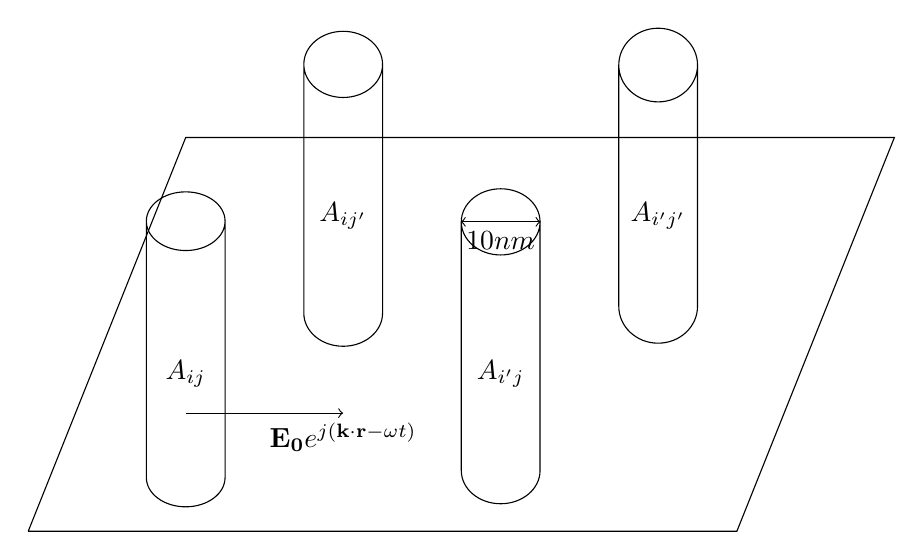
\begin{tikzpicture}
\node (A) at (1,0) [cylinder, shape border rotate=90, draw,minimum height=4cm,minimum width=1cm] {$A_{ij}$};
\node (B) at (5,0) [cylinder, shape border rotate=90, draw,minimum height=4cm,minimum width=1cm] {$A_{i'j}$};
\node (C) at (3,2) [cylinder, shape border rotate=90, draw,minimum height=4cm,minimum width=1cm] {$A_{ij'}$};
\node (D) at (7,2) [cylinder, shape border rotate=90, draw,minimum height=4cm,minimum width=1cm] {$A_{i'j'}$};
\draw (-1,-2) -- (8,-2) -- (10,3) -- (1,3) -- (-1,-2);
\draw [->] (1,-0.5) -- (3,-0.5) node[below] {$\mathbf{E_0}e^{j(\mathbf{k\cdot r} - \omega t)}$};
\draw [<->] (B.before top) -- (B.after top) node [midway, below] {$10nm$};
\end{tikzpicture}
\caption{Example of nano-cylinders embedded in dielectric.}
\label{fig:nano-cylinder}
\end{center}
\end{figure}

Analytical arguments are required to guarantee convergence and stability of the method, especially
in regimes which have strong nonlinear interaction.
Finally, although many techniques such as split-step Fourier method, $z$-transform,
NLSE (non-linear Schr{\"o}dinger equation) techniques~\cite{fibich2015nonlinear},
and spectral methods have been proposed, finite difference time domain method has remained the
computational work horse for the past decades. 
FDTD method has the advantage of simultaneous analysis of all the required frequency modes
in a single computation.
The FDTD method has been extended to handle
nonlinear media~\cite{joseph1997fdtd}, and parallel implementations have alleviated the computational costs~\cite{yu2006parallel}.
Nevertheless, full three-dimensional anisotropic nonlinear propagation of waves places
a significant computational burden. In this work, a discrete energy and momentum conserved
FDTD method for full three-dimensional analysis of nonlinear anisotropic media is presented.
Moreover, as we are analyzing dispersive and anisotropic media, numerical dispersion and
numerical anisotropic has to be carefully mitigated so as to not pollute the computational
result. This is a significant contribution of the present work. We present numerical results
validating our proposed method using examples from SHG, soliton propagation and self-focussing.

Recent work in the development of cylindrical gold nano-structures embedded in dielectric
has been shown to possess attractive optical properties which make them suitable for optical
computation,  a process which is based on light-light interaction and control of light using light.
Since experimental manufacture of such nano-materials is cost prohibitive and time consuming, a
numerical method which can analyze the optical behavior of nano-crystals with high accuracy and
efficiency is required.
Nano-crystals, especially Silicon Nitride has
very strong second harmonic generation (SHG), an area which has been
under analyzed due to the centro-symmetric nature of bulk silicon.

Consider the schematic of a nano-cylinder embedded in dielectric as shown in Figure~\ref{fig:nano-cylinder}.
The cylinders are mounted on fused silica substrate and the incident light wave is normal to the cylinder
surface. In addition to circular cylinders, elliptical cylinders and triangular prisms have also been
proposed.
Large third-order nonlinear optical susceptibility, $\chi^{(3)}$ has been reported for nanocomposites with 
gold (Au) and silver (Ag) nanoparticles~\cite{saonov1999nondegenerate,boyd2014third}. Similarly, second order
nonlinear optical susceptibility, $\chi^{(2)}$ has been reported for Silicon-nitride. As described 
by Boyd~\emph{et.~al.}, there are multiple contributors to the third-order nonlinear optical response, and
these can be classified as free-electron contribution, interband contribution and the hot-electron
contribution. The computed value is of the order of $10e^{-18}m^2/s^2$, and also it is important to note
that there is a delayed response component (of the order of 500fs). We highlight this example, as it 
represents a very challenging problem for 3d-FDTD due to the small timestep and large spatial domain.
Numerical results of our proposed scheme on this structure are presented in the sequel of this paper.

For the sequel of this paper we assume that polarization of the media (which may include nano-particles)
is available as a tensor of the form $\mathbf{P}^{(i)}(\omega,\mathbf{r},t)(\mathbf{E})$. It should be noted
that we are allowing for non-homogenous media, and for the polarization to be frequency and time dependent.
This allows for full flexibility in modeling delayed response, as well as resonance modes.  Photonic
bandgap software such as MPB~\cite{johnson2001block} can be used for this analysis.

\section{Problem Description}
\label{section:problem_description}
We begin, as is customary, by noting Maxwell's equations in vector differential form for anisotropic media
in a given domain $\Omega$ for a time duration $[0,T]$:
\begin{eqnarray}
\frac{\partial \mathbf{D}}{\partial t} + \mathbf{J} & = & \nabla \times \mathbf{H} \label{eqn:mx1}\\
\frac{\partial \mathbf{B}}{\partial t} & = & - \nabla \times \mathbf{E} \label{eqn:mx2}\\
\nabla \cdot \mathbf{D} & = & \rho \label{eqn:mx3}\\
\nabla \cdot \mathbf{B} & = & 0 \label{eqn:mx4} 
\end{eqnarray}
Here, $\mathbf{E}$ represents the electric field. We use the $j\omega t$ convention for
representing time varying fields, therefore, the electric field is $\mathbf{E}=\mathbf{E_0}e^{j\omega t}$.
Similarly, $\mathbf{H}$ represents the magnetic field. $\mathbf{D}$ represents the electric
displacement, and for nonlinear medium, its interaction with $\mathbf{E}$ is critical and analyzed
below in more detail. The magnetic displacement is denoted by $\mathbf{B}$. The current density
is denoted $\mathbf{J}$. Ohm's law:
\[
\mathbf{J} = \sigma \mathbf{E}
\]
where $\sigma$ is the electric conductivity, relates the conduction current density to the electric
field. The continuity of charge equation can be written as a differential equation:
\[
\frac{\partial \rho}{\partial t} + \nabla \cdot \mathbf{J} = 0
\]
Finally, the constitutive relation between magnetic flux and magnetic field can be written as:
\[
\mathbf{B} = \mu_0 \mathbf{H} + \mathbf{M}
\]
where $\mu_0$ is the free space permeability.
In the present work, we assume non-magnetic materials, and assume that the domain has no charges and
no conduction currents.
For ease of reference we note the following vector calculus identities and relations:
\begin{equation}
\nabla \cdot \mathbf{V} = \Big( \hat{\mathbf{i}} \frac{\partial}{\partial x}
+ \hat{\mathbf{j}} \frac{\partial}{\partial y}
+ \hat{\mathbf{k}} \frac{\partial}{\partial z} \Big) \cdot
\Big( V_x\hat{\mathbf{i}} + V_y\hat{\mathbf{j}} + V_z\hat{\mathbf{k}}\Big) =
\frac{\partial V_x}{\partial x} + 
\frac{\partial V_y}{\partial y} + 
\frac{\partial V_z}{\partial z} 
\end{equation}
\begin{equation}
\nabla \times \mathbf{V} = \begin{vmatrix}
\hat{\mathbf{i}} & \hat{\mathbf{j}} & \hat{\mathbf{k}} \\
\frac{\partial}{\partial x} & \frac{\partial}{\partial y} & \frac{\partial}{\partial z} \\
V_x & V_y & V_z
\end{vmatrix}
= \hat{\mathbf{i}}\Big( \frac{\partial V_z}{\partial y} - \frac{\partial V_y}{\partial z}\Big)
+ \hat{\mathbf{j}}\Big( \frac{\partial V_x}{\partial z} - \frac{\partial V_z}{\partial x}\Big)
+ \hat{\mathbf{k}}\Big( \frac{\partial V_y}{\partial x} - \frac{\partial V_x}{\partial y}\Big)
\end{equation}
\begin{equation}
\nabla \times ( \nabla \times \mathbf{V} ) = \nabla(\nabla \cdot \mathbf{V}) - 
\nabla^2\mathbf{V} \label{eqn:curl_curl}
\end{equation}

As an example of the use of the above identities, we can derive wave equation
corresponding to Maxwell's
equations. Take the curl of Equation~\ref{eqn:mx2}:
\begin{equation}
\nabla \times \nabla \times \mathbf{E} = - \frac{\partial}{\partial t} \nabla \times \mathbf{B}
= -\mu_0 \frac{\partial}{\partial t} \nabla \times H
= -\mu_0 \frac{\partial}{\partial t} \frac{\partial \mathbf{D}}{\partial t}
= -\mu_0 \epsilon_0 \frac{\partial^2 \mathbf{E}}{\partial t^2} \label{eqn:wave}
\end{equation}
where we use Equation~\ref{eqn:mx1}.
 Using the curl identity given in
Equation~\ref{eqn:curl_curl} as well as the divergence relation given in Equation~\ref{eqn:mx3}
we have
\begin{equation}
\frac{1}{c^2} \frac{\partial^2 \mathbf{E}}{\partial t^2} - \nabla^2\mathbf{E} = 0
\end{equation}
where $c=\frac{1}{\sqrt{\mu_0\epsilon_0}}$ is the speed of light in free space.

\subsection{Polarization }
\label{subsec:polarization}
In a linear medium, the electric displacement $\mathbf{D}$ and the electric field $\mathbf{E}$
are related as:
\begin{equation}
\mathbf{D} = \epsilon_0\mathbf{E} + \mathbf{P} \label{eqn:electric_displacement}
\end{equation}
where $\mathbf{P}$ is the electric polarization and $\epsilon_0$ is the free space permittivity.
The theory of electric polarization is well described in elementary electromagnetic books~\cite{balanis1999advanced}
and the theory of light propagation in dielectric solids is well explained in the book by Fowles~\cite{fowles1975introduction} and also the
book by Butcher and Cotter~\cite{butcher1991elements}. The material below is abstracted from the above sources. Consider a static electric field
applied to an isotropic medium (extension to the anisotropic case follow subsequently). Then, using a 
Lorentz-resonance model, each electron
in the dielctric medium is displaced from its original position by a distance $\mathbf{r}$. Assuming
an electron density of $N$ electrons in the volume, the total macroscopic polarization $\mathbf{P}$ is 
given by:
\begin{equation}
\mathbf{P} = N e \mathbf{r} \label{eqn:dipole_charge}
\end{equation}
where $e$ represents the electrical charge. When the electric field varies with time, the true
polarization is time dependent and is given as:
\[
m \frac{\partial^2 \mathbf{r}}{\partial t^2} + \gamma \frac{\partial \mathbf{r}}{\partial t} + K\mathbf{r} = e\mathbf{E}
\]
This is the differential equation of a harmonic oscillator. 
Dividing both sides by $m$, we have:
\[
\frac{\partial^2 \mathbf{r}}{\partial t^2} + \frac{\gamma}{m} \frac{\partial \mathbf{r}}{\partial t} + \frac{K}{m}\mathbf{r} = \frac{e}{m}\mathbf{E}
\]
As we have noted above, the electric field
is harmonic with frequency $\omega$, the above equation can be written as:
\[
\frac{\partial^2 \mathbf{r}}{\partial t^2} + \frac{\gamma}{m} \frac{\partial \mathbf{r}}{\partial t} + \frac{K}{m}\mathbf{r} = \frac{e}{m}\mathbf{E_0}e^{j\omega t}
\]
The general solution to the above equation can be written as $l_p(\omega,t) = l_0(\omega)e^{j\omega t}$, where
$l_0$ is the solution for $t=0$, which we can derive by substitution:
\[
l_0 = \frac{ \frac{e}{m} \mathbf{E_0}}{(\omega_0^2-\omega^2)+j\omega\frac{\gamma}{m}}
\]
where $\omega_0=\sqrt{\frac{K}{m}}$.
Assuming that there is no association in the molecules of the medium, the polarization $\mathbf{P}(\omega,t)$
can be written using Equation~\ref{eqn:dipole_charge} as:
\begin{equation}
\mathbf{P}(\omega,t) = \frac{ \frac{e^2}{m} \mathbf{E_0}e^{j\omega t}}{(\omega_0^2-\omega^2)+j\omega\frac{\gamma}{m}}
\label{eqn:polarization}
\end{equation}
The permittivity (witten as $\epsilon_0+\frac{\mathbf{P}}{\mathbf{E}}$) is therefore frequency dependent.
It should be noted that the permittivity is a complex number. If the medium has resonance at multiple frequencies
then the above equation for polarization has to be summed for each mode independently. We can expand
Equation~\ref{eqn:polarization} using a Taylor series in powers of $\mathbf{E}$, to get:
\begin{eqnarray}
\mathbf{P} & = & \mathbf{\chi}^{(1)}(\mathbf{E}) + \mathbf{\chi}^{(2)}(\mathbf{E}\otimes\mathbf{E}) + \mathbf{\chi}^{(3)}(\mathbf{E}\otimes\mathbf{E}\otimes\mathbf{E}) + \ldots \nonumber \\
           & = & \mathbf{P}^{(1)} + \mathbf{P}^{(2)} + \mathbf{P}^{(3)} + \ldots \label{eqn:nonlinear-polarization}
\end{eqnarray}
where $\mathbf{\chi}$ is a tensor coefficient, called the electric susceptibility. 
The book by Butcher and Cotter~\cite{butcher1991elements}~pp.~16, clearly
explains the use of tensor contraction in writing $\mathbf{P}^{(2)}$ as:
\begin{eqnarray}
\mathbf{P}^{(2)} & = & \epsilon_0 \int_{-\infty}^\infty d\tau_1 \int_{-\infty}^\infty d\tau_2 \mathbf{R}^{(2)} (t-\tau_1, t-\tau_2): \mathbf{E}(\tau_1) \mathbf{E}(\tau_2) \\
& = & \epsilon_0 \int_{-\infty}^\infty d\tau'_1 \int_{-\infty}^\infty d\tau'_2 \mathbf{R}^{(2)} (\tau'_1, \tau'_2): \mathbf{E}(t-\tau_1) \mathbf{E}(t-\tau_2) 
\end{eqnarray}
In the above equations, $\mathbf{R}^{(2)}$ is the quadratic polarization
response tensor of the medium, and the equations capture the time-invariance,
causality and \emph{intrinsic permutation symmetry} of the
polarization. Generalizations to $n=3$ are immediate, and it should be
noted that $\mathbf{R}$ then becomes a $(n+1)$ rank tensor.
Therefore we can now
write the electric displacement constitutive equation, Equation~\ref{eqn:electric_displacement} as:
\begin{equation}
\mathbf{D} = \mathbf{P}^{(1)}\mathbf{E} + \mathbf{P}^{(2)}\mathbf{E} + \mathbf{P}^{(3)}\mathbf{E} 
\label{eqn:electric_displacement_2}
\end{equation}
Next, we consider the dispersiveness of the medium; the linear polarization $\mathbf{P}^{(1)}$ can
be written as the sum of an instantenous response (corresponding to $\omega=\infty$) and a
dispersive response:
\begin{equation}
\mathbf{P}^{(1)} = \mathbf{P}^{(1)}_{\infty}(\mathbf{E}) + \mathbf{P}^{(1)}_{\mathrm{disp}}(\mathbf{E}) \label{eqn:electric_displacement_3}
\end{equation}
The dispersive response can be modelled using a Lorentz bi-modal resonance model. 
As in~\cite{bourgeade_and_nkonga_siam_2005}, define $\mathbf{P}^{(1)}_\mathrm{disp}$ as:
\begin{equation}
\mathbf{P}^{(1)}_\mathrm{disp}(\mathbf{E}) = \alpha_a \mathbf{F} + \alpha_b \mathbf{G} \label{eqn:alpha_a_b}
\end{equation}
where $\alpha_a$ and $\alpha_b$ are second-order tensors, such that $\alpha_a+\alpha_b = I_d$.
The Lorentz material
model is written as:
\begin{equation}
\epsilon(\omega) = \epsilon_0\epsilon_\infty + \epsilon_0 \sum_{p=1}^P \frac{(\epsilon_{s,p}-\epsilon_{\infty,p})\omega_p^2}
{\omega_p^2 + 2j\omega - \omega^2}
\label{eqn:lorentz_material}
\end{equation}
where $\epsilon_{s,p}$ is the permittivity at zero frequency, $\epsilon_{\infty,p}$ is the
permittivity as $\omega$ approaches inifinity, and $\omega_p$ is the resonant frequency of
the medium. 
We can use rational complex functions to represent the $\epsilon(\omega)$ dependence:
\[
\epsilon(\omega) = \epsilon_0\epsilon_\infty + \sum_{p=1}^P \frac{A_p}{\omega-W_p}
\]
where $W_p$ are complex poles, and $A_p$ is a complex resonance mode dependent coefficient.
We can therefore express the permittivity $\epsilon$ in the time domain as:
\[
\epsilon(t) = \epsilon_0\epsilon_\infty + \epsilon_0\chi(t)
\]
Susceptibility tensors can also be analyzed using Fourier techniques by writing the electric field
as:
\begin{equation}
\mathbf{E}(t,\mathbf{r}) = \int_{-\infty}^\infty d\omega \int_{-\infty}^\infty d\mathbf{k} \quad
\mathbf{E}(\omega,\mathbf{k}) \exp[-i(\mathbf{k}\cdot\mathbf{r} - \omega t)]
\end{equation}
Now, the susceptibility tensors depend not only on the incident frequency, but also on the optical wave
vectors $\mathbf{k}$. We can write it as (following~\cite{butcher1991elements}):
\begin{eqnarray}
\mathbf{P}^{(n)}(t,\mathbf{r}) & = & \epsilon_0 \int_{-\infty}^\infty d\omega_1 \int_{-\infty}^\infty d\omega_2 \ldots \int_{-\infty}^\infty d\omega_n
\int_{-\infty}^\infty d\mathbf{k}_1 \int_{-\infty}^\infty d\mathbf{k}_2 \ldots \int_{-\infty}^\infty d\mathbf{k}_n \nonumber \\
& & \times\ \mathbf{\chi}^{(n)}(-\omega_{\sigma};\omega_1,\mathbf{k}_1,\omega_2,\mathbf{k}_2,\ldots,\omega_n,\mathbf{k}_n)|
\mathbf{E}(\omega_1,\mathbf{k}_1)\mathbf{E}(\omega_2,\mathbf{k}_2)\cdots\mathbf{E}(\omega_n,\mathbf{k}_n) \\
& & \times \exp[-i(\mathbf{k}_P\cdot\mathbf{r}-\omega_{\sigma}t)] \nonumber %\label{eqn:polarization-n}
\end{eqnarray}
where $\omega_{\sigma}=\sum_{j=1}^n \omega_j$ and $\mathbf{k}_P = \sum_{j=1}^n \mathbf{k}_j$, and
the vertical bar $|$, denotes $n$-variable tensor contraction.
The response tensor $\mathbf{R}^{(n)}$ is used in $\mathbf{\chi}^{(n)}$:
\begin{eqnarray}
\mathbf{\chi}^{(n)}(-\omega_{\sigma};\omega_1,\mathbf{k}_1,\omega_2,\mathbf{k}_2,\ldots,\omega_n,\mathbf{k}_n) & = &
\int_{-\infty}^\infty d\tau_1 \int_{-\infty}^\infty d\tau_2 \ldots \int_{-\infty}^\infty d\tau_n
\int_{-\infty}^\infty d\mathbf{r}_1 \int_{-\infty}^\infty d\mathbf{r}_2 \ldots \int_{-\infty}^\infty d\mathbf{r}_n \nonumber \\
& & \times\ \mathbf{R}^{(n)}(\tau_1,\mathbf{r}_1,\tau_2,\mathbf{r}_2,\dots,\tau_n,\mathbf{r}_n)
\exp[i \sum_{j=1}^n(\mathbf{k}_j\cdot\mathbf{r}_j-\omega_j\tau_j)] \nonumber
\end{eqnarray}
In both equations above, the intrinsic permutation symmetry implies that each term is counted
only once in its symmetric form. 

For anisotropic crystals, where the principal optical axis is aligned with the laboratory
coordinates, Bourgeade and Nkonga, present a simplified model in~\cite{bourgeade_and_nkonga_siam_2005}.
\textbf{TO DO: Please derive these equations}
Using the formulae in~\cite{bourgeade_and_nkonga_siam_2005}, the dispersive linear polarization
$\mathbf{P}^{(1)}_\mathrm{disp}$ is characterized by two Lorentz resonances (indexed by $a$ and $b$):
\begin{eqnarray}
\frac{\partial^2 \mathbf{F}}{\partial t^2} + \delta_a \frac{\partial \mathbf{F}}{\partial t} + 
\omega_a^2 \mathbf{F} & = & \omega^2_a\cdot\mathbf{\chi}_d\cdot\mathbf{E} \\
\frac{\partial^2 \mathbf{G}}{\partial t^2} + \delta_b \frac{\partial \mathbf{G}}{\partial t} + 
\omega_b^2 \mathbf{G} & = & \omega^2_b\cdot\mathbf{\chi}_d\cdot\mathbf{E}  \label{eqn:lorentz}
\end{eqnarray}
where $\omega_a$ and $\omega_b$ are angular verilocity tensors associated with the Lorentz frequencies,
$\delta_a$ and $\delta_b$ are the corresponding damping tensors, and $\chi_d$ is a material specific
tensor, which highlights the optical property of the material. 
For now, we use isotropic medium (therefore $\chi_d$ is scalar), 
but we will extend the results to anisotropic media as well
in the sequel.
We will use example of uniaxial
crystals for the numerical experiments.
For simplicity of notation we introduce two scalars $\beta$ and $\gamma$ (defined below)
which are used in the non-linear dispersion equations in isotropic medium.
\begin{equation}
\mathbf{P}^{(2)}(\mathbf{E}) = \begin{pmatrix} 
d_{14} & \mathbf{E}_y & \mathbf{E}_z \\
d_{14} & \mathbf{E}_x & \mathbf{E}_z \\
d_{36} & \mathbf{E}_x & \mathbf{E}_y 
\end{pmatrix}
\end{equation}
Then $\beta=d_{14}$.
Similarly we define $\mathbf{P}^{(3)}(\mathbf{E})$, and $\gamma$ is
the entry in the tensor. Therefore we can write the polarization as
\begin{equation}
D = \epsilon_0(\epsilon_\infty E_x + \alpha_a F + \alpha_b G + \beta E^2 + \gamma E^3) \label{eqn:main-polarization}
\end{equation}

It should be noted that using finite difference methods for deriving the polarization
may not be the most efficient method for nano-crystals, since the number of grid points
required for accurate simulation can easily exceed 10,000. Therefore, we believe that a hybrid
method of using Fourier techniques for deriving $\mathbf{P}(\omega)$ combined with a FDTD method
for propagating $\mathbf{E}$ and $\mathbf{H}$ is required.

\subsection{Anisotropic Medium}
\label{subsec:anisotropic-medium}
In this section we describe the properties of uniaxial and biaxial medium, especially the
properties of birefringence and the generation of second harmonic (SHG). As we describe below,
the anisotropic medium has a coordinate system, denoted the \emph{principal optical axis}, there
the permittivity of the medium can be represented as a diagonal tensor. It should be noted, that this
coordinate system need not be aligned with the laboratory coordinate system and a coordinate rotation
needs to be applied when analyzing the problem. Generally this is implemented as:
\[
u(\mathbf{r},t) = R^{-1}(\theta,\psi) U(\mathbf{r},t) R(\theta,\psi)
\]

\begin{enumerate}
\item Scalar equation for polarization
\item Principal axis, $k$-vector, energy direction, $D,E,S$
\item Birefringence
\item Index plots (circle and ellipse), positive and negative materials, phase matching, and quasi-phase matching
\item Second harmonic generation
\end{enumerate}

\subsection{Homogenous Medium}
To begin with, we have considerd homogenous medium. However, an interesting study can be
done combining the work of defect distributions in the crystal and their impact on the optical
properties. Similarly, the manufacturability of nano-crystals is not defect free, and their
defect density can be modeled. In our implementation, we have used $\epsilon(\omega,\mathbf{r},t)$ to model
the frequency, position and time dependence of our permittivity tensor.

\subsection{Problem definition}
Given an initial excited incident wave, numerically propagate the wave through the nonlinear
medium $\Omega$ for the time duraction $T$.

\section{Previous Work}
\label{sec:previous_work}
The above problem has been solved for the anisotropic and nonlinear case previously.
Standard introduction to the field of optics including non-linear optics,
polarization and plane wave solutions to Maxwell's equations are given in~\cite{boyd2012contemporary,agrawal2007nonlinear,fowles1975introduction}.
A classical text on nonlinear optics is Zernike and Midwinter~\cite{zernike2006applied} and
Butcher and Cotter~\cite{butcher1991elements}.
Bourgeade and Nkonga present a numerical method for second harmonic
generation modeling of laser pulses in anisotropic nonlinear crystal 
KDP~\cite{bourgeade_and_nkonga_siam_2005}. 
An energy stable discontinuous Galerkin method was presented by
Bokil~\emph{et. al.} in~\cite{BOKIL2017420}, and operator splitting based methods
are presented in~\cite{BOKIL2014160}.
Recently, Sakkaplangkul has presented a novel operator splitting
scheme for Maxwell's equation in linear non-dispersive and
non-dissipative material, as well as ferromagnetic material.
High order methods including fourth order methods are presented in~\cite{YEFET2001286, energy_conserved_siam_2010,
Chen2008,bokil2011analysis}.
A good introduction to finite difference time domain (FDTD) methods
is given by Joseph and Taflove in~\cite{joseph1997fdtd}, and Taflove and Hagness~\cite{taflove2005computational}
as well
as the books~\cite{yu2006parallel,rylander2012computational,leveque2007finite}. 
Numerical wave propagation algorithms are discussed by Cohen in~\cite{cohen2001higher,cohen2016finite}.
Algorithms in this work are
implemented using the Julia programming language~\cite{bezanson2017julia}.
The author has presented
symbolic methods for analyzing silicon photonic waveguides 
in~\cite{koranneTCAD_Photonics}.

\subsection{The Yee staggered grid for FDTD}
\label{subsec:yee}

\begin{figure}
\begin{center}
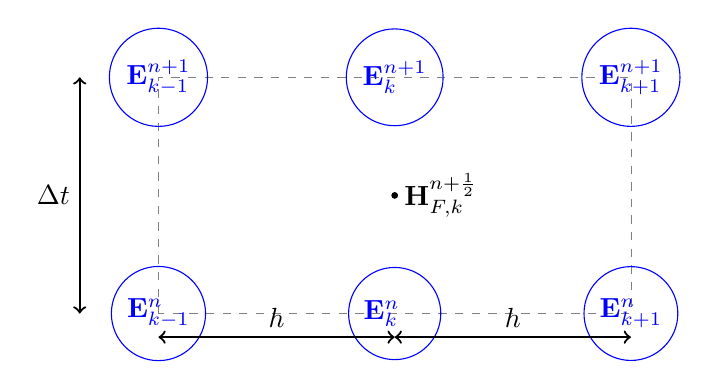
\begin{tikzpicture}
\draw[mgrid] (0,0) rectangle (6,3);
\node[mpoint] at (0,0) {$\mathbf{E}^n_{k-1}$};
\node[mpoint] at (3,0) {$\mathbf{E}^n_{k\quad}$};
\node[mpoint] at (6,0) {$\mathbf{E}^n_{k+1}$};  

\node[mpoint] at (0,3) {$\mathbf{E}^{n+1}_{k-1}$};
\node[mpoint] at (3,3) {$\mathbf{E}^{n+1}_{k\quad}$};
\node[mpoint] at (6,3) {$\mathbf{E}^{n+1}_{k+1}$};  

\draw[fill] (3,1.5) circle(1pt)  node[anchor=west] {$\mathbf{H}^{n+\frac{1}{2}}_{F,k}$};
\draw[thick,<->] (0,-0.3) -- (3,-0.3) ;
\draw[] (1.5,-0.3) node[anchor=south] {$h$};
\draw[thick,<->] (3,-0.3) -- (6,-0.3) ;
\draw[] (4.5,-0.3) node[anchor=south] {$h$};

\draw[thick,<->] (-1,0) -- (-1,3) ;
\draw[] (-1,1.5) node[anchor=east] {$\Delta t$};


\end{tikzpicture}
\caption{The classical Yee staggered grid for 1D.}
\label{fig:yee-1D}
\end{center}
\end{figure}

We first write the vector Maxwell's equation in 3d component form.
\begin{equation}
\mu\frac{\partial \mathbf{H}}{\partial t} =  - \nabla \times \mathbf{E} \\
%\frac{\partial \mathbf{D}}{\partial t} & = & \nabla \times \mathbf{H} \\
\end{equation}
%We can use $c_0=\frac{1}{\sqrt{\epsilon_0\mu_0}}$, where $c_0$ is the speed of light in vaccum.
\begin{eqnarray}
\frac{\partial E_z}{\partial y} - \frac{\partial E_y}{\partial z} & = & -\big( \mu_{xx} \frac{\partial H_x}{\partial t}  + \mu_{xy} \frac{\partial H_y}{\partial t}  + \mu_{xz} \frac{\partial H_z}{\partial t}  \big)  \\
\frac{\partial E_x}{\partial z} - \frac{\partial E_z}{\partial x} & = & -\big( \mu_{yx} \frac{\partial H_x}{\partial t}  + \mu_{yy} \frac{\partial H_y}{\partial t}  + \mu_{yz} \frac{\partial H_z}{\partial t}  \big)  \\
\frac{\partial E_y}{\partial x} - \frac{\partial E_x}{\partial y} & = & -\big( \mu_{zx} \frac{\partial H_x}{\partial t}  + \mu_{zy} \frac{\partial H_y}{\partial t}  + \mu_{zz} \frac{\partial H_z}{\partial t}  \big)  
\end{eqnarray}

Assuming that the permeability tensor is symmetric, we can simplify the above
equations as:
\begin{eqnarray}
\frac{\partial E_z}{\partial y} - \frac{\partial E_y}{\partial z} & = & - \mu_{xx} \frac{\partial H_x}{\partial t}  \label{eqn:maxwell-component-begin} \\
\frac{\partial E_x}{\partial z} - \frac{\partial E_z}{\partial x} & = & - \mu_{yy} \frac{\partial H_y}{\partial t} \\
\frac{\partial E_y}{\partial x} - \frac{\partial E_x}{\partial y} & = & - \mu_{zz} \frac{\partial H_z}{\partial t} 
\end{eqnarray}

Next consider the relation between electric displacement and curl of the
magnetic field.
\begin{equation}
\frac{\partial \mathbf{D}}{\partial t}  =  \nabla \times \mathbf{H} \nonumber
\end{equation}
We can expand this into component form as:
\begin{eqnarray}
\frac{\partial H_z}{\partial y} - \frac{\partial H_y}{\partial z} & = & \epsilon_0 \big( \epsilon_{xx} \frac{\partial D_x}{\partial t}  + \epsilon_{xy} \frac{\partial D_y}{\partial t}  + \epsilon_{xz} \frac{\partial D_z}{\partial t}  \big) \\
\frac{\partial H_x}{\partial z} - \frac{\partial H_z}{\partial x} & = & \epsilon_0 \big( \epsilon_{yx} \frac{\partial D_x}{\partial t}  + \epsilon_{yy} \frac{\partial D_y}{\partial t}  + \epsilon_{yz} \frac{\partial D_z}{\partial t}  \big)  \\
\frac{\partial H_y}{\partial x} - \frac{\partial H_x}{\partial y} & = & \epsilon_0 \big( \epsilon_{zx} \frac{\partial D_x}{\partial t}  + \epsilon_{zy} \frac{\partial D_y}{\partial t}  + \epsilon_{zz} \frac{\partial D_z}{\partial t}  \big)  \label{eqn:maxwell-component-end}
\end{eqnarray}

The relation between $\mathbf{D}$ and $\mathbf{E}$ is given above in
Equation~\ref{eqn:electric_displacement_2}, and we substitute it above to get:
\begin{eqnarray}
\frac{\partial H_z}{\partial y} - \frac{\partial H_y}{\partial z} & = & \epsilon_0 \Big( \epsilon_{xx} \frac{\partial (P^{(1)}_xE_x+P^{(2)}_xE_yE_z+P^{(3)}_xE_xE_yE_z)}{\partial t}  \nonumber \\
& & + \epsilon_{xy} \frac{\partial (P^{(1)}_yE_y+P^{(2)}_yE_xE_z+P^{(3)}_yE_xE_yE_z)}{\partial t}  \nonumber \\
& & + \epsilon_{xz} \frac{\partial (P^{(1)}_zE_z+P^{(2)}_zE_xE_y+P^{(3)}_zE_xE_yE_z)}{\partial t}  \Big) 
\end{eqnarray}
\begin{eqnarray}
\frac{\partial H_x}{\partial z} - \frac{\partial H_z}{\partial x} & = & \epsilon_0 \Big( \epsilon_{yx} \frac{\partial (P^{(1)}_xE_x+P^{(2)}_xE_yE_z+P^{(3)}_xE_xE_yE_z)}{\partial t}  \nonumber \\
& & + \epsilon_{yy} \frac{\partial (P^{(1)}_yE_y+P^{(2)}_yE_xE_z+P^{(3)}_yE_xE_yE_z)}{\partial t}  \nonumber \\
& & + \epsilon_{yz} \frac{\partial (P^{(1)}_zE_z+P^{(2)}_zE_xE_y+P^{(3)}_zE_xE_yE_z)}{\partial t}  \Big) 
\end{eqnarray}
\begin{eqnarray}
\frac{\partial H_y}{\partial x} - \frac{\partial H_x}{\partial y} & = & \epsilon_0 \Big( \epsilon_{zx} \frac{\partial (P^{(1)}_xE_x+P^{(2)}_xE_yE_z+P^{(3)}_xE_xE_yE_z)}{\partial t}  \nonumber \\
& & + \epsilon_{zy} \frac{\partial (P^{(1)}_yE_y+P^{(2)}_yE_xE_z+P^{(3)}_yE_xE_yE_z)}{\partial t}  \nonumber \\
& & + \epsilon_{zz} \frac{\partial (P^{(1)}_zE_z+P^{(2)}_zE_xE_y+P^{(3)}_zE_xE_yE_z)}{\partial t}  \Big)
\end{eqnarray}

Next, we use Equation~\ref{eqn:electric_displacement_3} and substitute the dispersive relations in the
above equations. At this time, we make a simplification, and only consider 1D wave propagation. The full extension
for 2D and 3D is done subsequently. We assume that that wave is propagating in the $z$-direction, 
with the electric field in the $x$ direction (so, $E_y=0$) and the magnetic field in the $y$ direction,
(so, $H_x=0$),
and assume no
variation in the $x$ and $y$ directions, either for the field or the parameters. Moreover, we also assume
isotropic medium for this analysis.
Therefore all derivatives with respect to the $x$ and $y$ variables, are set to zero. Then we get the following
simplified set of equations:
\begin{eqnarray}
\frac{\partial E_x}{\partial z} & = & - \mu_{yy} \frac{\partial H_y}{\partial t} \\
- \frac{\partial H_y}{\partial z} & = & \epsilon_0 \Big( \epsilon_{xx} \frac{\partial (P^{(1)}_xE_x+P^{(2)}_xE^2_x+P^{(3)}_xE^3_x)}{\partial t} \Big) \\
& = & \epsilon_0 \Big( \epsilon_{xx}\frac{\partial ((P^{(1)}_\infty)_xE_x+(P^{(1)}_\mathrm{disp})_xE_x)+P^{(2)}_xE^2_x+P^{(3)}_xE^3_x)}{\partial t} \Big) 
\end{eqnarray}
We can use the Lorentz form for $\mathbf{P}^{(1)}_\mathrm{disp}$ as $\mathbf{F}$ and $\mathbf{G}$ as shown in
Equation~\ref{eqn:alpha_a_b}, to get:
\begin{eqnarray}
\frac{\partial E_x}{\partial z} & = & - \mu_{yy} \frac{\partial H_y}{\partial t} \\
- \frac{\partial H_y}{\partial z} & = & \epsilon_0 \Big( \epsilon_{xx}\frac{\partial ((P^{(1)}_\infty)_xE_x+(\alpha_aF_x+\alpha_bG_x)+P^{(2)}_xE^2_x+P^{(3)}_xE^3_x)}{\partial t} \Big) 
\end{eqnarray}
We discretize the above equations using finite difference in 1D below, using the Yee
grid as shown in Figure~\ref{fig:yee-1D}.
%Consider the Yee grid for 1D FDTD as shown in Figure~\ref{fig:yee-1D}.

\begin{figure}
\begin{center}
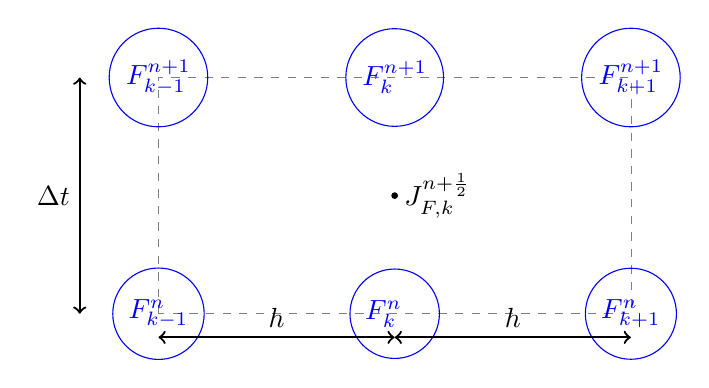
\begin{tikzpicture}
\draw[mgrid] (0,0) rectangle (6,3);
\node[mpoint] at (0,0) {$F^n_{k-1}$};
\node[mpoint] at (3,0) {$F^n_{k\quad}$};
\node[mpoint] at (6,0) {$F^n_{k+1}$};  

\node[mpoint] at (0,3) {$F^{n+1}_{k-1}$};
\node[mpoint] at (3,3) {$F^{n+1}_{k\quad}$};
\node[mpoint] at (6,3) {$F^{n+1}_{k+1}$};  

\draw[fill] (3,1.5) circle(1pt)  node[anchor=west] {$J^{n+\frac{1}{2}}_{F,k}$};
\draw[thick,<->] (0,-0.3) -- (3,-0.3) ;
\draw[] (1.5,-0.3) node[anchor=south] {$h$};
\draw[thick,<->] (3,-0.3) -- (6,-0.3) ;
\draw[] (4.5,-0.3) node[anchor=south] {$h$};

\draw[thick,<->] (-1,0) -- (-1,3) ;
\draw[] (-1,1.5) node[anchor=east] {$\Delta t$};


\end{tikzpicture}
\caption{Proposed finite difference discretization scheme for $J_F$ in 1D.}
\label{fig:1D-scheme}
\end{center}
\end{figure}

\section{Proposed Algorithm}
\label{section:proposed_algorithm}
We first explain the proposed method using 1D, extension to 2D and 3D are given subsequently.
We use a staggered grid finite difference time domain method to solve the above problem.
Let $h$ denote the spatial grid resolution (we begin by making the spatial grid resolution fixed, and
equal in all dimensions). Let $\Delta t$ denote the time resolution, as derived from the CFL~\cite{taflove2005computational} condition. We divide the problem into phases, and in the first phase we discretize the electric
displacement and polarization using Equation~\ref{eqn:lorentz}. In~\cite{bourgeade_and_nkonga_siam_2005}
the authors have used a three-step second-order accurate scheme to calculate $\mathbf{F}^{n+1}$.
We, however, present a simplification by calculating the polarization current $\mathbf{J}_F$
and $\mathbf{J}_G$, using a first-order method as described below:
\begin{eqnarray}
\frac{\partial \mathbf{F}}{\partial t} & = & \mathbf{J}_F \label{eqn:lorentz-first-order-begin} \\
\frac{\partial \mathbf{J}_F}{\partial t} + \delta_a \mathbf{J}_F + \omega^2_a \mathbf{F}& = & \omega^2_a \cdot \chi_d \cdot \mathbf{E}  \\
\frac{\partial \mathbf{G}}{\partial t} & = & \mathbf{J}_G  \\
\frac{\partial \mathbf{J}_G}{\partial t} + \delta_b \mathbf{J}_G + \omega^2_b \mathbf{G} & = & \omega^2_b \cdot \chi_d \cdot \mathbf{E} \label{eqn:lorentz-first-order-end}
\end{eqnarray}
The proposed finite difference scheme for $\mathbf{J}_F$ in 1D is shown in Figure~\ref{fig:1D-scheme}.
Note that $\mathbf{E}$ and $\mathbf{H}$ are staggered as in the Yee-scheme~\cite{taflove2005computational}, but
$\mathbf{F},\mathbf{J}_F,\mathbf{G},\mathbf{J}_G$ are discretized like $\mathbf{E}$ in space and time.
An alternative approach would be discretize $\mathbf{J}_F,\mathbf{F}$ like $\mathbf{E}$ in space
but discretize $\mathbf{J}_F$ like $\mathbf{H}$ in time, and $\mathbf{F}$ like $\mathbf{E}$ in time.
The value for $\mathbf{J}_F$ is calculated at $t=n+\frac{1}{2}$, while $\mathbf{F}$ is calculated at
$x=kh,t=n\Delta t$, and is written as $\mathbf{F}_{k}^n$. To calculate, $\mathbf{J}_{F,k}^{n+\frac{1}{2}}$, we
use time averaging:
\begin{equation}
\frac{ \mathbf{F}^{n+1}_k - \mathbf{F}^n_k}{\Delta t} = \frac{\mathbf{J}_{F,k}^{n+1}+\mathbf{J}_{F,k}^n}{2}
\end{equation}
Similarly, for $\mathbf{J}_G$, we have:
\begin{equation}
\frac{ \mathbf{G}^{n+1}_k - \mathbf{G}^n_k}{\Delta t} = \frac{\mathbf{J}_{G,k}^{n+1}+\mathbf{J}_{G,k}^n}{2}
\end{equation}
Substituting the above in the Lorentz equations, Equations~\ref{eqn:lorentz-first-order-begin}--\ref{eqn:lorentz-first-order-end}, we have:
\begin{eqnarray}
\frac{ \mathbf{J}^{n+1}_{F,k} - \mathbf{J}^n_{F,k}}{\Delta t} + \delta_a \frac{\mathbf{J}_{F,k}^{n+1}+\mathbf{J}_{F,k}^n}{2}
+ \omega^2_a \frac{\mathbf{F}_{k}^{n+1}+\mathbf{F}_{k}^n}{2} & = & \omega^2_a \cdot \chi_d \cdot 
\frac{\mathbf{E}^{n+1}_k+\mathbf{E}^n_k}{2} \\
\frac{ \mathbf{J}^{n+1}_{G,k} - \mathbf{J}^n_{G,k}}{\Delta t} + \delta_b \frac{\mathbf{J}_{G,k}^{n+1}+\mathbf{J}_{G,k}^n}{2}
+ \omega^2_b \frac{\mathbf{G}_{k}^{n+1}+\mathbf{G}_{k}^n}{2} & = & \omega^2_b \cdot \chi_d \cdot 
\frac{\mathbf{E}^{n+1}_k+\mathbf{E}^n_k}{2} 
\end{eqnarray}

Assuming 1D spatial dimensions, We can write the difference equations for $\mathbf{H}$ and $\mathbf{E}$:
\begin{eqnarray}
\frac{H_{y,j+\frac{1}{2}}^{n+\frac{1}{2}} - H_{y,j+\frac{1}{2}}^{n-\frac{1}{2}}}{\Delta t} & = & -\mu_{yy}
\frac{E_{x,j+1}^{n} - E_{x,j}^{n}}{\Delta x} \\
\frac{D_{x,j}^{n+1} - D_{x,j}^{n}}{\Delta t} & = & \frac{H_{y,j+\frac{1}{2}}^{n+\frac{1}{2}} - H_{y,j-\frac{1}{2}}^{n+\frac{1}{2}}}{\Delta y}
\end{eqnarray}

\section{Energy Analysis}
\label{section:energy_analysis}
Given a nonlinear anisotropic medium $\Omega$, with periodic boundary conditions for all fields, the 
nonlinear Maxwell's equations given above satisfy the following energy identity.
\begin{thm}[Energy Identity]
Given $\Omega$, with periodic boundary conditions:
\[
\frac{d}{dt} E(t) = -\int_{\partial\Omega} (E\times H)\cdot \mathbf{n}\ d\sigma 
- \epsilon_0 \int_\Omega \Big( (\frac{\sqrt{\alpha_a\delta_a}\mathbf{F}}{\omega_a\sqrt{\chi_d}})^2 +
(\frac{\sqrt{\alpha_b\delta_b}\mathbf{G}}{\omega_b\sqrt{\chi_d}})^2 \Big) dz
\]
where $E(t)$ is given by:
\[
E(t) = \frac{1}{2} \int_\Omega \Big(\mu_0\mathbf{H}^2 + \epsilon_0\epsilon_\infty \mathbf{E}^2 
 + \frac{\epsilon_0\alpha_a\mathbf{J_F}^2}{\chi_d\omega^2_a} 
+ \frac{\epsilon_0\alpha_a\mathbf{F}^2}{\chi_d}
+ \frac{\epsilon_0\alpha_b\mathbf{J_G}^2}{\chi_d\omega^2_b} 
+ \frac{\epsilon_0\alpha_b\mathbf{G}^2}{\chi_d}
+\frac{2}{3}\epsilon_0\beta \mathbf{E}^3
+\frac{3}{4}\epsilon_0\gamma \mathbf{E}^4
\Big)\ dz
\]
\end{thm}
\begin{proof}
We prove the identity for 1D case, the proof for 2D and 3D follows similarly and is given
in the sequel of this paper. For a wave propagating in the $z$ direction, we are given:
\begin{eqnarray}
\mu_0 \frac{\partial H_y}{\partial t} & = & \frac{\partial E_x}{\partial z} \label{eqn:id0} \\
\frac{\partial D}{\partial t} & = & \frac{\partial H_y}{\partial z} \label{eqn:id1} \\
D & = & \epsilon_0(\epsilon_\infty E_x + \alpha_a F + \alpha_b G + \beta E^2 + \gamma E^3) \label{eqn:id2}
\end{eqnarray}
where $\beta$ is instantaneous contribution due to $\mathbf{P}^{(2)}$ and 
$\gamma$ is instantaneous contribution due to $\mathbf{P}^{(3)}$.
The constitutive relationship between $\mathbf{F}$ and $\mathbf{E}$ (similarly for
$\mathbf{G}$ and $\mathbf{E}$) is given by Equation~\ref{eqn:lorentz}, and we can write that 
second order differential equation in first order to avoid instability due to incorrect
time centering~\cite{gilles2000comparison}.
%% \begin{eqnarray}
%% \frac{\partial \mathbf{F}}{\partial t} & = & \mathbf{J_F} \label{eqn:id3} \\
%% \frac{\partial \mathbf{J_F}}{\partial t} + \delta_a\mathbf{J_F} + \omega^2_a\mathbf{F} & = & \omega^2_a \chi_d \mathbf{E} \label{eqn:id4} \\
%% \frac{\partial \mathbf{G}}{\partial t} & = & \mathbf{J_G} \label{eqn:id5} \\
%% \frac{\partial \mathbf{J_G}}{\partial t} + \delta_b\mathbf{J_G} + \omega^2_b\mathbf{G} & = & \omega^2_b \chi_d \mathbf{E} \label{eqn:id6}
%% \end{eqnarray}
Substitute Equation~\ref{eqn:id2} into Equation~\ref{eqn:id1}, to get:
\begin{equation}
\frac{\partial}{\partial t} \epsilon_0 ( \epsilon_\infty E + \alpha_a F + \alpha_b G + \beta E^2 + \gamma E^3) = 
\frac{\partial H}{\partial z} \label{eqn:id7}
\end{equation}
Using Equations~\ref{eqn:id0} by $H$, Equation~\ref{eqn:id7} by $E$ and adding together we get:
\begin{equation}
\mu_0 H \frac{\partial H}{\partial t} + E \frac{\partial}{\partial t} \epsilon_0 ( \epsilon_\infty E + \alpha_a F + \alpha_b G + \beta E^2 + \gamma E^3) = H \frac{\partial E}{\partial z} + E \frac{\partial H}{\partial z} 
\label{eqn:id8}
\end{equation}
Since $\frac{\partial F}{\partial t} = J_F$ and $\frac{\partial G}{\partial t} = J_G$, we have 
\begin{eqnarray}
\frac{1}{2}\epsilon_0 \frac{\partial F^2}{\partial t} & = & \epsilon_0 F\ J_F \label{eqn:id7b} \\
\frac{1}{2}\epsilon_0 \frac{\partial G^2}{\partial t} & = & \epsilon_0 G\ J_G \label{eqn:id7c} 
\end{eqnarray}

Multiplying Equations~\ref{eqn:lorentz-first-order-begin} by $\frac{J_F\epsilon_0}{\omega^2_a}$ and Equation~\ref{eqn:id8} by
$\frac{J_G\epsilon_0}{\omega^2_b}$, and using Equation~\ref{eqn:id7b} and Equation~\ref{eqn:id7c}:
\begin{eqnarray}
\frac{\epsilon_0}{\omega^2_a} J_F \frac{\partial J_F}{\partial t} & = &
-\frac{\epsilon_0\delta_a J_F^2}{\omega^2_a} - \epsilon_0 J_F F + \epsilon_0 \chi_d J_F \mathbf{E} \label{eqn:id9}\\
\frac{\epsilon_0}{\omega^2_b} J_G \frac{\partial J_G}{\partial t} & = &
-\frac{\epsilon_0\delta_b J_G^2}{\omega^2_b} - \epsilon_0 J_G G + \epsilon_0 \chi_d J_G \mathbf{E} \label{eqn:id10}\\
\frac{1}{2} \frac{\partial}{\partial t}[\frac{\epsilon_0}{\omega^2_a} J_F^2 + \epsilon_0 F^2] & = & \epsilon_0 \chi_d E\ J_F - \frac{\epsilon_0\delta_a J_F^2}{\omega^2_a} \label{eqn:id11} \\
\frac{1}{2} \frac{\partial}{\partial t}[\frac{\epsilon_0}{\omega^2_b} J_G^2 + \epsilon_0 G^2] & = & \epsilon_0 \chi_d E\ J_G - \frac{\epsilon_0\delta_b J_G^2}{\omega^2_b} \label{eqn:id12} 
\end{eqnarray}
Therefore, $\epsilon_0 E\ J_F$ can be written as:
\begin{equation}
\epsilon_0 E\ J_F = \frac{1}{2} \frac{\epsilon_0}{\chi_d} \frac{\partial}{\partial t}[\frac{J_F^2}{\omega^2_a}  + F^2] + \frac{\epsilon_0\delta_a J_F^2}{\omega^2_a} \label{eqn:id13} 
\end{equation}
Similarly,
\begin{equation}
\epsilon_0 E\ J_G = \frac{1}{2} \frac{\epsilon_0}{\chi_d} \frac{\partial}{\partial t}[\frac{J_G^2}{\omega^2_b}  + G^2] + \frac{\epsilon_0\delta_b J_G^2}{\omega^2_b} \label{eqn:id14} 
\end{equation}
We can also write, $\epsilon_0 \beta E \frac{\partial}{\partial t}E^2$ as
\[
\epsilon_0 \beta E \frac{\partial}{\partial t}E^2 = \frac{2}{3} \epsilon_0 \beta \frac{\partial }{\partial t} E^3
\]
and
\[
E \frac{\partial}{\partial t} \epsilon_0 \gamma E^3 = \frac{3}{4} \epsilon_0 \gamma \frac{\partial}{\partial t}E^4
\]
Substituting in Equation~\ref{eqn:id8} we get:
\begin{equation}
\frac{1}{2} \frac{\partial}{\partial t}\Big[\mu_0\mathbf{H}^2 + \epsilon_0\epsilon_\infty \mathbf{E}^2 
+\frac{2}{3}\epsilon_0\beta \mathbf{E}^3
+\frac{3}{4}\epsilon_0\gamma \mathbf{E}^4
\Big] + \epsilon_0\alpha_a E\ J_F + \epsilon_0\alpha_b E\ J_G = \frac{\partial}{\partial z}(E\times H)\label{eqn:id15}
\end{equation}
Substituting from Equation~\ref{eqn:id13} and Equation~\ref{eqn:id14} into Equation~\ref{eqn:id15}, we get
the required identity using the periodic boundary conditions on $\Omega$.
\end{proof}

\subsection{Travelling wave propagation}
\label{subsec:plane-wave}
Next we consider the propagation of a linearly polarized 1D plane wave, $\mathbf{E}=E(z,t)$ propagating
in the $z$-direction. 
Then the form of the wave is:
\[
\mathbf{E}(\mathbf{r},t) = E_x(\mathbf{r},t)\hat{i} = \{E_0(z,t)\exp[i(kz-\omega t)]+\mathrm{c.c.}\}\hat{i}
\]
The other fields such as $\mathbf{H},\mathbf{P},\mathbf{D}$, therefore also have
the same form. Using the travelling wave assumption, we can write the above fields in $\xi=z-vt$ 
coordinate. 
\begin{thm}[Travelling Wave Propagation]
Given $\mathbf{E}$ as above, the coupled system of polarization $\mathbf{P}$ and $\mathbf{E}$ has
stationary point at $(E,W)=(0,0)$, where $W=\frac{\partial E}{\partial \xi}$.
The system has additional stationary points at:
\begin{eqnarray}
(E,W) & = & (\frac{\omega_0^2 (\frac{-\beta}{\sqrt{\gamma}}\sqrt{\frac{c^2}{v^2}-\epsilon_s} + 2\frac{c^2}{v^2} - 2\epsilon_s)}
{v^2(\frac{\beta}{\sqrt{\gamma}}\sqrt{\frac{c^2}{v^2}-\epsilon_s} + 3\epsilon_s - \epsilon_\infty) - 2c^2},0)
\end{eqnarray}
and
\begin{eqnarray}
(E,W) & = & (\frac{\omega_0^2 (\frac{\beta}{\sqrt{\gamma}}\sqrt{\frac{c^2}{v^2}-\epsilon_s} + 2\frac{c^2}{v^2} - 2\epsilon_s)}
{v^2(\frac{-\beta}{\sqrt{\gamma}}\sqrt{\frac{c^2}{v^2}-\epsilon_s} + 3\epsilon_s - \epsilon_\infty) - 2c^2},0)
\end{eqnarray}
\end{thm}
\begin{proof}
Substituting in the Maxwell's equation we get:
\begin{eqnarray}
\mu_0 \frac{\partial H}{\partial t} & = & \frac{\partial E}{\partial z} \\
\frac{\partial H}{\partial z} & = & \frac{\partial D}{\partial t} \\
D & = & \epsilon_0( \epsilon_\infty E + \alpha_a F + \alpha_b G + \beta E^2 + \gamma E^3) \label{eqn:D_pol}\\
\frac{\partial D}{\partial t} & = & \epsilon_0( \epsilon_\infty \frac{\partial E}{\partial t} + 
\alpha_a \frac{\partial F}{\partial t}
+ \alpha_b \frac{\partial G}{\partial t}
+2\beta E \frac{\partial E}{\partial t} + 3\gamma E^2\frac{\partial E}{\partial t}) \label{eqn:D_by_dt}
\end{eqnarray}

Using the chain rule we have the following relations:
\begin{eqnarray}
\xi & = & z - vt \\
E(z,t) & = & E(\xi) \\
\frac{\partial E}{\partial \xi} & = & W \\
\frac{\partial E}{\partial z} & = & \frac{\partial E}{\partial \xi} \frac{\partial \xi}{\partial z} = \frac{\partial E}{\partial \xi} = W \\
\frac{\partial E}{\partial t} & = & \frac{\partial E}{\partial \xi} \frac{\partial \xi}{\partial t} = -vW \\
\frac{\partial^2 E}{\partial t^2} & = & \frac{\partial}{\partial t} (-vW) = -v \frac{\partial W}{\partial t} = -v \frac{\partial W}{\partial \xi}\frac{\partial \xi}{\partial t} = v^2 \frac{\partial W}{\partial \xi} \\
\frac{\partial D}{\partial \xi} & = & -\frac{1}{v} \frac{\partial H}{\partial \xi} = 
\frac{1}{\mu_0 v^2}\frac{\partial E}{\partial \xi} \implies D = \frac{1}{\mu_0 v^2} E\label{eqn:Deqn}
\end{eqnarray}

To compute $\frac{\partial W}{\partial \xi}$, we use the chain-rule and Equation~\ref{eqn:lorentz},
as follows:
\begin{eqnarray}
\frac{\partial W}{\partial \xi} & = & \frac{\partial}{\partial \xi} ( \frac{\partial E}{\partial \xi}) \\
& = & \frac{\partial}{\partial \xi} ( \frac{\partial E}{\partial z}) = \frac{\partial}{\partial \xi} \mu_0 \frac{\partial H}{\partial t} = \frac{\partial}{\partial t} \mu_0 \frac{\partial H}{\partial \xi} 
= \frac{\partial}{\partial t} \mu_0 \frac{\partial H}{\partial z} = \mu_0 \frac{\partial^2 D}{\partial t^2}\\
& = & \frac{1}{c^2} \Big( -v\epsilon_\infty \frac{\partial W}{\partial t} + (\alpha_a \frac{\partial^2 F}{\partial t^2}
+ \alpha_b \frac{\partial^2 G}{\partial t^2}) + \frac{\partial }{\partial t}(2\beta E\frac{\partial E}{\partial t})
+ \frac{\partial }{\partial t}(3\gamma E^2\frac{\partial E}{\partial t})\Big)\\
& = & \frac{1}{c^2} \Big( v^2\epsilon_\infty \frac{\partial W}{\partial \xi} + (\alpha_a \frac{\partial^2 F}{\partial t^2}
+ \alpha_b \frac{\partial^2 G}{\partial t^2}) + 2 \beta E \frac{\partial^2 E}{\partial t^2} + 
2\beta (\frac{\partial E}{\partial t})^2 + 3\gamma E^2 \frac{\partial^2 E}{\partial t^2} +
6\gamma E (\frac{\partial E}{\partial t})^2\Big) \nonumber \\
& = & \frac{1}{c^2} \Big( v^2\epsilon_\infty \frac{\partial W}{\partial \xi} + (\alpha_a \frac{\partial^2 F}{\partial t^2}
+ \alpha_b \frac{\partial^2 G}{\partial t^2}) + 2 \beta E v^2 \frac{\partial W}{\partial \xi}
+ 2\beta (-vW)^2 + 3\gamma E^2 v^2 \frac{\partial W}{\partial \xi} + 6\gamma E (-vW)^2 \nonumber \Big) \\
& = & \frac{1}{c^2} \Big( v^2\epsilon_\infty \frac{\partial W}{\partial \xi} + (\alpha_a \frac{\partial^2 F}{\partial t^2}
+ \alpha_b \frac{\partial^2 G}{\partial t^2}) + 2 \beta E v^2 \frac{\partial W}{\partial \xi}
+ 2 \beta v^2 W^2 + 3\gamma E^2 v^2 \frac{\partial W}{\partial \xi} + 6\gamma E v^2W^2 \nonumber \Big) 
\end{eqnarray}

As in previous work~\cite{sorensen2005kink}, we have 
assumed $\delta_a$ and $\delta_b$ to be zero, as when $\omega$ is near
the resonance frequency, the damping terms can be ignored, and we get
\[
\delta_a = \delta_b = 0 \implies \frac{\partial^2 F}{\partial t^2} = \omega_a^2(\chi_d E - F)
\]
Similarly, for $G$
\[
\frac{\partial^2 G}{\partial t^2} = \omega_b^2(\chi_d E - G)
\]
Now since $F$ and $G$ are the \emph{linear} dispersive polarization, we can calculate them
separately and superimpose. 
Using Equation~\ref{eqn:D_pol} and Equation~\ref{eqn:Deqn}:
\begin{eqnarray}
\alpha_a F & = & \frac{E}{\mu_0\epsilon_0 v^2} - \epsilon_\infty E - \beta E^2 - \gamma E^3 \\
\alpha_b G & = & \frac{E}{\mu_0\epsilon_0 v^2} - \epsilon_\infty E - \beta E^2 - \gamma E^3
\end{eqnarray}
Substituting from the above equations, and using $\mu_0\epsilon_0 c^2=1$, we get:
\begin{eqnarray}
\alpha_a \frac{\partial^2 F}{\partial t^2} + \alpha_b \frac{\partial^2 G}{\partial t^2} & = &
\alpha_a\omega_a^2(\chi_d E - F) + \alpha_b\omega_b^2(\chi_d E - G) \nonumber \\
& = & \alpha_a\omega_a^2\chi_d E - \omega_a^2( \frac{Ec^2}{v^2} - \epsilon_\infty E -
 \beta E^2 - \gamma E^3)
+\alpha_b\omega_b^2\chi_d E -\omega_b^2 (\frac{Ec^2}{v^2} - 
\epsilon_\infty E - \beta E^2 - \gamma E^3) \nonumber\\
& = & E\omega_a^2(\alpha_a\chi_d - \frac{c^2}{v^2}+\epsilon_\infty +\beta E + 
\gamma E^2) + 
E\omega_b^2(\alpha_b\chi_d - \frac{c^2}{v^2}+\epsilon_\infty +\beta E + 
\gamma E^2)
\end{eqnarray}
Substituting above in the equation for $\frac{\partial W}{\partial \xi}$, we get:
\begin{eqnarray}
\frac{\partial W}{\partial \xi}[1-\frac{1}{c^2}(\epsilon_\infty v^2 + 2\beta Ev^2 + 3\gamma E^2 v^2)] & = &
\frac{1}{c^2}\Big( 2\beta v^2W^2 + 6\gamma E v^2 W^2 \nonumber \\
& & - E\omega_a^2[\frac{c^2}{v^2} - \alpha_a \chi_d 
- \epsilon_\infty  - \beta E -\gamma E^2] \nonumber \\
& & - E\omega_b^2[\frac{c^2}{ v^2} - \alpha_b \chi_d 
- \epsilon_\infty  - \beta E -\gamma E^2]\Big)
\end{eqnarray}
Rearranging:
\begin{eqnarray}
\frac{\partial E}{\partial \xi} & = & W \nonumber \\
\frac{\partial W}{\partial \xi} & = & \frac{6\gamma E v^2 W^2 +2\beta v^2W^2
 - E\omega_a^2[\frac{c^2}{v^2}-\alpha_a \chi_d  
- \epsilon_\infty  - \beta E -\gamma E^2] 
 - E\omega_b^2[\frac{c^2}{v^2} - \alpha_b \chi_d  
- \epsilon_\infty  - \beta E -\gamma E^2]}
{c^2 - v^2(\epsilon_\infty +2\beta E + 3\gamma E^2)}\nonumber \\% \label{eqn:mykink}
& = & \frac{6\gamma E v^2 W^2 +2\beta v^2W^2
-E\omega_0^2[\frac{c^2}{v^2} - \epsilon_s  -\beta E -\gamma E^2]}
{c^2 - v^2(\epsilon_\infty +2\beta E + 3\gamma E^2)} \label{eqn:mykink}
\end{eqnarray}
where we have denoted
\[
\omega_0^2 = \omega_a^2 + \omega_b^2
\]
and
\[
\epsilon_s = \chi_d\frac{\alpha_a\omega_a^2 + \alpha_b\omega_b^2}{\omega_0^2} + \epsilon_\infty
\]

We should note that above Equation~\ref{eqn:mykink} is very similar to the derivation
by Sorensen and Webb~\cite{sorensen2005kink}, where they have only considered
the cubic nonlinearity and their Lorentz dispersion term only consists of
a single component, while we have used the Sellemeir relation~\cite{bourgeade_and_nkonga_siam_2005} which gave us
$\alpha_a F+\alpha_b G$.
We see that $(E,W)=(0,0)$ is a stationary point of this system.
Let $E_\infty$ and $W_\infty$, denote the stationary points of the system, and let $f$ and $g$ represent the
right hand side functions of Equation~\ref{eqn:mykink}, respectively.
Using the theory of dynamical systems, we can write the above system of equations as:
\[
\frac{d}{d\xi}\begin{bmatrix} E \\ W \end{bmatrix} = A \begin{bmatrix} E \\ W \end{bmatrix}
\]
where $A$ is given as
\[
A = \begin{bmatrix} f_E(E_\infty,W_\infty) & f_W(E_\infty,W_\infty)\\
                    g_E(E_\infty,W_\infty) & g_W(E_\infty,W_\infty) \end{bmatrix}
\]
where $f_E$, $f_W$ and $g_E$ and $g_W$ are the elements of the Jacobian, evaluated
at the stationary points. The eigenvalues of this Jacobian yield information about
the dynamical behavior of the system\footnote{Especially using the
Hartman-Grobman Theorem, we can predict the behavior of the
linearized system near the critical points.}. Writing the Jacobian at 
$(E_\infty,W_\infty)=(0,0)$, we get
\[
A = \begin{bmatrix} 0 & 1 \\
                    \frac{\omega_0^2[\frac{c^2}{v^2} - \epsilon_s]}
                    {\epsilon_\infty v^2-c^2} & 0 
\end{bmatrix}
\]
Calculating the eigenvalues of $A$, we get 
\[
\lambda^2 =\frac{\omega_0^2[\frac{c^2}{v^2} - \epsilon_s]}
                    {\epsilon_\infty v^2 - c^2} 
\]
Therefore we get:
\begin{equation}
\lambda = \pm i \omega_0 \sqrt{ \frac{ \frac{c^2}{v^2} -\epsilon_s }
{c^2-\epsilon_\infty v^2}} \label{eqn:caseI}
\end{equation}
Substituting the values and $E=0,W=0.001$, we plot the phase plot as shown
in Figure~\ref{fig:caseI}(b). Since the eigenvalues are complex, we can see the
oscillation around the stationary point $(0,0)$.

The system has additional stationary points which can be calculated by solving
the above system simultaneously. We continue to postulate $W_\infty=0$, so
that the first two terms of $\frac{\partial W}{\partial \xi}$ become
zero, and only the terms which have $E\omega_0^2$
as leading factors have to be analyzed.
To analyze the stationary points we
solve for the quadratic in $E$

\begin{equation}
\gamma E^2 + \beta E - K = 0
\end{equation}
where $K=\frac{c^2}{v^2}-\epsilon_s$.
Solving for $E$, we get
\[
E_\infty = \frac{ -\beta \pm \sqrt{\beta^2 + 4\gamma K}}{2\gamma}
\]

To calculate the eigenvalues of the system at these stationary points, we have
to compute the Jacobian at this point.
\[
A = \begin{bmatrix} \frac{\partial W}{\partial E}|_{E_\infty} & \frac{\partial W}{\partial W}|_{W_\infty=0} \\
\frac{\partial g}{\partial E}|_{E_\infty} & \frac{\partial g}{\partial W}|_{W_\infty=0}
\end{bmatrix}
\]
where $g(E,W)$ is the function representing $\frac{\partial W}{\partial \xi}$.
Thus
\begin{eqnarray}
g_E|E_\infty & = & \frac{\partial}{\partial E}\ \frac{-E \omega_0^2 [ -\gamma E^2 - \beta E + K ]}
{c^2 - v^2(\epsilon_\infty +2\beta E + 3\gamma E^2)}\\
& = & \frac{ E_\infty\omega_0^2 (2\gamma E_\infty + \beta ) }
{c^2 - v^2(\epsilon_\infty +2\beta E_\infty + 3\gamma E_\infty^2)}
\end{eqnarray}
Here we note that when $E=E_\infty$,
\[
3\gamma E^2 + 2\beta E = (\gamma E^2 + \beta E - K) + 2\gamma E^2 + \beta E + K
= 2\gamma E^2 + \beta E + K
\]
Substituting above:
\begin{eqnarray}
g_E|E_\infty & = & \frac{ \omega_0^2 E_\infty(2\gamma E_\infty + \beta ) }
{c^2 - v^2(E_\infty(2\gamma E_\infty + \beta) + \epsilon_\infty + \frac{c^2}{v^2}-\epsilon_s)} \\
& = & \frac{\omega_0^2}
{-v^2(1+\frac{\epsilon_\infty - \epsilon_s}{E_\infty(2\gamma E_\infty + \beta)})} \label{eqn:maineqn}
\end{eqnarray}
Note that $2\gamma E_\infty + \beta =\pm \sqrt{\beta^2+4\gamma K}$; we choose the positive square root first
\[
2\gamma E_\infty + \beta = \sqrt{\beta^2 + 4\gamma K}
\]
Utilizing the fact that $\beta \ll 1$, we can simplify further to get:
\[
E_\infty ( \sqrt{\beta^2 + 4\gamma K}) = \frac{(-\beta \pm \sqrt{\beta^2+4\gamma K})}{2\gamma} \sqrt{\beta^2 + 4\gamma K} = \frac{-\beta}{\sqrt{\gamma}}\sqrt{\frac{c^2}{v^2}-\epsilon_s}
\pm 2(\frac{c^2}{v^2}-\epsilon_s)
\]
Thus
\begin{eqnarray}
E_\infty ( 2\gamma E_\infty + \beta ) & = & (\frac{-\beta + \sqrt{\beta^2 + 4\gamma K}}{2\gamma})\sqrt{\beta^2 + 4\gamma K} \\
& = & \frac{-\beta}{\sqrt{\gamma}}\sqrt{\frac{c^2}{v^2}-\epsilon_s} + 2(\frac{c^2}{v^2}-\epsilon_s)\label{eqn:pos}
\end{eqnarray}

Similarly for the conjugate root:
\begin{equation}
2\gamma E_\infty + \beta = -\sqrt{\beta^2 + 4\gamma K}
\end{equation}
Substituting into the above equation

\begin{eqnarray}
E_\infty ( 2\gamma E_\infty + \beta ) & = & (\frac{\beta + \sqrt{\beta^2 + 4\gamma K}}{2\gamma})\sqrt{\beta^2 + 4\gamma K} \\
& = & \frac{\beta}{\sqrt{\gamma}}\sqrt{\frac{c^2}{v^2}-\epsilon_s} + 2(\frac{c^2}{v^2}-\epsilon_s) \label{eqn:neg}
\end{eqnarray}
Substituting from Equation~\ref{eqn:pos} into Equation~\ref{eqn:maineqn}
\begin{eqnarray}
g_E|E_\infty & = & \frac{\omega_0^2}
{-v^2(1+\frac{\epsilon_\infty - \epsilon_s}{E_\infty(2\gamma E_\infty + \beta)})} \\
& = & \frac{\omega_0^2 (\frac{-\beta}{\sqrt{\gamma}}\sqrt{\frac{c^2}{v^2}-\epsilon_s} + 2\frac{c^2}{v^2} - 2\epsilon_s)}
{-v^2(\frac{-\beta}{\sqrt{\gamma}}\sqrt{\frac{c^2}{v^2}-\epsilon_s} + 2(\frac{c^2}{v^2} - \epsilon_s) + \epsilon_\infty - \epsilon_s)} \\
& = & \frac{\omega_0^2 (\frac{-\beta}{\sqrt{\gamma}}\sqrt{\frac{c^2}{v^2}-\epsilon_s} + 2\frac{c^2}{v^2} - 2\epsilon_s)}
{v^2(\frac{\beta}{\sqrt{\gamma}}\sqrt{\frac{c^2}{v^2}-\epsilon_s} + 3\epsilon_s - \epsilon_\infty) - 2c^2} \label{eqn:complex1}
\end{eqnarray}
%\chi_d\frac{\alpha_a\omega_a^2 + \alpha_b\omega_b^2}{\omega_0^2}
As a check, we substitute $\beta=0$ in the above equation, to get
\[
g_E|(E_\infty,\beta=0) = 2\omega_0^2\frac{\frac{c^2}{v^2}-\epsilon_s}
{v^2(3 \epsilon_s - \epsilon_\infty) -2c^2} 
\]
Again this equation matches the result given in~\cite{sorensen2005kink}.
Next we substitute Equation~\ref{eqn:neg} into Equation~\ref{eqn:maineqn}
\begin{eqnarray}
g_E|E_\infty & = & \frac{\omega_0^2}
{-v^2(1+\frac{\epsilon_\infty - \epsilon_s}{E_\infty(2\gamma E_\infty + \beta)})} \\
& = & \frac{\omega_0^2 (\frac{\beta}{\sqrt{\gamma}}\sqrt{\frac{c^2}{v^2}-\epsilon_s} + 2\frac{c^2}{v^2} - 2\epsilon_s)}
{-v^2(\frac{\beta}{\sqrt{\gamma}}\sqrt{\frac{c^2}{v^2}-\epsilon_s} + 2(\frac{c^2}{v^2} - \epsilon_s) + \epsilon_\infty - \epsilon_s)} \\
& = & \frac{\omega_0^2 (\frac{\beta}{\sqrt{\gamma}}\sqrt{\frac{c^2}{v^2}-\epsilon_s} + 2\frac{c^2}{v^2} - 2\epsilon_s)}
{v^2(\frac{-\beta}{\sqrt{\gamma}}\sqrt{\frac{c^2}{v^2}-\epsilon_s} + 3\epsilon_s - \epsilon_\infty) - 2c^2} \label{eqn:real1}
\end{eqnarray}

Using the above Equation~\ref{eqn:complex1} and Equation~\ref{eqn:real1}, we get
\[
\frac{c^2}{v^2} - \epsilon_s > 0 \implies |v| < \frac{c}{\sqrt{\epsilon_s}}
\]
Similarly,
\begin{equation}
v^2(\frac{\beta}{\sqrt{\gamma}}\sqrt{\frac{c^2}{v^2}-\epsilon_s} + 3\epsilon_s - \epsilon_\infty) - 2c^2 > 0
\end{equation}
Combine the above to get
\begin{equation}
c\sqrt{\frac{2}{\frac{\beta}{\sqrt{\gamma}}\sqrt{\frac{c^2}{v^2}-\epsilon_s} + 3\epsilon_s - \epsilon_\infty}}  < |v| <  \frac{c}{\sqrt{\epsilon_s}} \label{eqn:ineq}
\end{equation}
In this region, if $v$ is chosen appropriately as follows:
\[
\frac{-\beta}{\sqrt{\gamma}}\sqrt{\frac{c^2}{v^2}-\epsilon_s} + 2\frac{c^2}{v^2} - 2\epsilon_s < 0
\]

Substituting from Equation~\ref{eqn:complex1} in $A$:
\[
A = \begin{bmatrix} 0 & 1 \\
\frac{\omega_0^2 (\frac{-\beta}{\sqrt{\gamma}}\sqrt{\frac{c^2}{v^2}-\epsilon_s} + 2\frac{c^2}{v^2} - 2\epsilon_s)}
{v^2(\frac{\beta}{\sqrt{\gamma}}\sqrt{\frac{c^2}{v^2}-\epsilon_s} + 3\epsilon_s - \epsilon_\infty) -2c^2}& 0
\end{bmatrix}
\]
Computing the eigenvalues of $A$, we have

\begin{eqnarray}
\lambda & = & \pm \sqrt{\frac{\omega_0^2 (\frac{-\beta}{\sqrt{\gamma}}\sqrt{\frac{c^2}{v^2}-\epsilon_s} + 2\frac{c^2}{v^2} - 2\epsilon_s)}
{v^2(\frac{\beta}{\sqrt{\gamma}}\sqrt{\frac{c^2}{v^2}-\epsilon_s} + 3\epsilon_s - \epsilon_\infty) -2c^2}} \label{eqn:caseII}
\end{eqnarray}
These eigenvalues and the corresponding stationary points are analyzed below in Case II.
The other set of eigenvalues are calculated similarly, to be:
\begin{eqnarray}
\lambda & = & \pm \sqrt{\frac{\omega_0^2 (\frac{\beta}{\sqrt{\gamma}}\sqrt{\frac{c^2}{v^2}-\epsilon_s} + 2\frac{c^2}{v^2} - 2\epsilon_s)}
{v^2(\frac{-\beta}{\sqrt{\gamma}}\sqrt{\frac{c^2}{v^2}-\epsilon_s} + 3\epsilon_s - \epsilon_\infty) -2c^2}} \label{eqn:caseIII}
\end{eqnarray}
These eigenvalues and the corresponding stationary points are analyzed below in Case III.
\end{proof}

\section{Stability analysis using Lyapunov energy function}
At the non-hyperbolic stationary point, the stability analysis for the non-linear equation requires care, as the linearization
from the Jacobian may not necessarily carry over. We use energy estimates of $E^2+W^2$ to conclude that at $(E,W)=(0,0)$, the
stationary point is asymptotically stable. We consider a Lyapunov function $r(\xi)=E^2+W^2$, and the plot for various initial
conditions for case I (with purely imaginary eigenvalues) is shown in Figure~\ref{fig:CY1}.

\begin{figure}[htb]
\begin{center}
\subfigure[$(E,W)=(0,0)$]{\includegraphics[width=4.6cm]{C1LY0}}
\subfigure[$(E,W)=(2,0)$]{\includegraphics[width=4.6cm]{C1LY2}}
\subfigure[$(E,W)=(-0.8,0)$]{\includegraphics[width=4.6cm]{C1LYM2}}
\caption{Lyapunov function $r(\xi)=E^2+W^2$ plot for case I.}
\label{fig:CY1}
\end{center}
\end{figure}



We also verify this with numerical simulation in the second part of this section.
At the hyperbolic point, as the analysis suggests, for the negative Real eigenvalue, the phase plot show a inward spiral, and 
at the positive real eigenvalue, an unstable equilibrium.

For the third case, when the analysis is regime dependent on $v$, for certain values of $v$, the eigenvalues switch from
real to complex and we can perform the Hopf bifurcation analysis. A comprehensive numerical simulation plot is shown in
Figure~\ref{fig:numerical_phase_plot}.

\subsection{Hopf Bifurcation Analysis}
As shown above we have three stationary points, and as we verify with numerical simulations, the stationary points
are stable only at certain parameter values of $v$. 
This analysis depends on the location of the eigenvalues
as well as satisfying the criteria for Hopf bifurcation. 
\[
\lambda = \pm i \omega_0 \sqrt{ \frac{ \frac{c^2}{v^2} -\epsilon_s }
{c^2-\epsilon_\infty v^2}}
\]
We can see that for the case of $(E,W)=(0,0)$, both eigenvalues are complex, moreover $\mathrm{Re}\frac{d\lambda}{dv}=0$, therefore
the criteria for Hopf bifurcation is not met, and we conclude that there is no Hopf bifurcation at this stationary point.
Plotting the dependence of the $E/W$ phase plot on $v$ confirms this behavior near the stationary point as shown
in Figure~\ref{fig:vdep}. We can see that although there is a continuous dependence on $v$, there is no bifurcation.

\begin{figure}[htb]
\begin{center}
\includegraphics[width=15cm]{PLOTS/EW_V}
\caption{Dependence of the phase plot on $v$ parameter.}
\label{fig:vdep}
\end{center}
\end{figure}

Plotting Equation~\ref{eqn:caseI}, as shown in Figure~\ref{fig:caseI}, we observe that at $v=0.6652$, 
\begin{figure}[htb]
\begin{center}
\subfigure[Case I: eigenvalues of $A$ as a function of $v$]{\includegraphics[width=8.5cm]{case1_zoom_in_hopf}}
\subfigure[Phase plot for Case I]{\includegraphics[width=6cm]{PLOTS/EW_V6_5}}
\caption{Case I: eigenvalues of $A$ as a function of $v$.}
\label{fig:caseI}
\end{center}
\end{figure}

\begin{figure}[htb]
\begin{center}
\subfigure[Phase plot for $E,W$]{\includegraphics[width=4.6cm]{PLOTS/EW_phase_plot}}
\subfigure[Plot of $E$ vs $\xi$]{\includegraphics[width=4.6cm]{ME19}}
\subfigure[Plot of $W$ vs $\xi$]{\includegraphics[width=4.6cm]{MW19}}
\caption{Phase plot of $E,W$ around $(0,0)$}
\label{fig:ME19}
\end{center}
\end{figure}




\section{Refractive Index}
\label{sec:refractive-index}
Using Equation~\ref{eqn:mykink} the effective refractive index can be computed from the dispersion relations as follows.
Consider the plane wave given as $E=E_0\exp^{i(\mathbf{k}-\omega t)}$, where the relation between $\omega$ and $\mathbf{k}$ is
given as $D(\omega,\mathbf{k})=0$. Then using Fourier analysis $\frac{\partial}{\partial t}=-i\omega$ and
$\frac{\partial}{\partial \mathbf{x}}=i\mathbf{k}$ (we can use this technique on the non-linear polarization
equation, provided $\mathbf{k}$ is close to $\mathbf{k_0}$).
\begin{thm}[Refractive index]
The refractive index of a medium considering non-linear polarization is given as
\begin{equation}
n^2 = \chi^{(1)}(\omega) = c^2\frac{k^2}{\omega^2} = \epsilon_\infty + \frac{\alpha_a \chi_d}{1-(\frac{\omega}{\omega_a})^2} + \frac{\alpha_b \chi_d}{1-(\frac{\omega}{\omega_b})^2} \label{eqn:refindex1}
\end{equation}
when damping is zero. When the damping term is included we have
\begin{equation}
n^2 = \epsilon_\infty + \frac{\alpha_a \chi_d}{1-(\frac{\omega}{\omega_a})^2-i\frac{\omega}{\omega_a}\delta_a'} 
+ \frac{\alpha_a \chi_d}{1-(\frac{\omega}{\omega_b})^2-i\frac{\omega}{\omega_b}\delta_b'} 
\end{equation}
where $\delta_a'=\frac{\delta_a}{\omega}$ and $\delta_b'=\frac{\delta_b}{\omega}$, are the normalized damping terms.
\end{thm}
\begin{proof}
Consider the Lorentz equations given above in Equation~\ref{eqn:lorentz}, and using the Fourier multiplication rule for plane wave (as the 
Lorentz polarization also follows the plane wave polarization of $E$), we have
\begin{eqnarray}
-\omega^2 F - i\omega\delta_a F + \omega_a^2 F & = & \omega_a^2 \cdot \chi_d \cdot \mathbf{E} \nonumber \\
-\omega^2 G - i\omega\delta_b G + \omega_b^2 G & = & \omega_b^2 \cdot \chi_d \cdot \mathbf{E} 
\end{eqnarray}
Therefore
\begin{eqnarray}
\alpha_a \frac{F}{\mathbf{E}} & = & \frac{\alpha_a \chi_d}{1-(\frac{\omega}{\omega_a})^2-i\frac{\omega}{\omega_a}\delta_a'} \nonumber \\
\alpha_b \frac{G}{\mathbf{E}} & = & \frac{\alpha_b \chi_d}{1-(\frac{\omega}{\omega_b})^2-i\frac{\omega}{\omega_b}\delta_b'} \label{eqn:refindex-fg}
\end{eqnarray}
where $\delta_a'=\frac{\delta_a}{\omega}$ and $\delta_b'=\frac{\delta_b}{\omega}$, are the normalized damping terms.
Next consider the equation for polarization $D$ given above in Equation~\ref{eqn:main-polarization}, and substituting it in the Maxwell's equation we have
\begin{eqnarray}
\mu_0\frac{\partial H}{\partial t} & = & \frac{\partial E}{\partial z} \implies \mu_0(-i\omega)H = i k E \implies \mu_0 k H = \frac{-k^2}{\omega}E \nonumber \\
\frac{\partial H}{\partial z} & = & \frac{\partial D}{\partial t} \implies i k H = (-i \omega) D \nonumber \\
\mu_0 (k H) & = & -\mu_0 \omega D = \frac{-k^2}{\omega} E \nonumber
\end{eqnarray}
Combine to get
\begin{eqnarray}
\omega^2 \mu_0 D - k^2 E & = & 0 \nonumber \\
\frac{\omega^2}{c^2}(\epsilon_\infty E + \alpha_a F + \alpha_b G + \beta E^2 + \gamma E^3) - k^2 E & = & 0 \nonumber \\
\Big[\omega^2(\epsilon_\infty + \frac{\alpha_a F}{E} + \frac{\alpha_b G}{E} + \beta |E| + \gamma |E|^2) - c^2 k^2\Big] E & = & 0 \nonumber \\
\omega^2 \chi^{(1)}(\omega) - c^2 k^2 & = & 0 \label{eqn:refindex-main-eqn}
\end{eqnarray}
Where, using Equation~\ref{eqn:refindex-fg} and Equation~\ref{eqn:refindex-main-eqn}, we can write $\chi^{(1)}(\omega)$ as
\[
\chi^{(1)}(\omega) = \frac{c^2 k^2}{\omega^2} = \epsilon_\infty + \frac{\alpha_a \chi_d}{1-(\frac{\omega}{\omega_a})^2-i\frac{\omega}{\omega_a}\delta_a'}
+ \frac{\alpha_b \chi_d}{1-(\frac{\omega}{\omega_b})^2-i\frac{\omega}{\omega_b}\delta_b'} 
\]
By setting the damping term to zero, we get the result.
\end{proof}

\subsection{Group Velocity}
The group velocity can be calculated from the above relation $D(\omega,\mathbf{k})$.
\begin{thm}[Group velocity]
Consider the plane wave given as $E=E_0\exp^{i(\mathbf{k}-\omega t)}$, where the relation between $\omega$ and $\mathbf{k}$ is
given as $D(\omega,\mathbf{k})=0$. Then the group velocity, denoted, $v_g$, can be calculated as
\[
v_g = \frac{c^2k}{ \frac{2\alpha_a \chi_d \omega_a^2 \omega^2}{(\omega_a^2-\omega^2)^2} + 
\frac{2\alpha_b \chi_d \omega_b^2 \omega^2}{(\omega_b^2-\omega^2)^2} }
\]
\end{thm}
\begin{proof}
We know from~\cite{brio2010numerical}, that the group velocity is calculated as
\[
v_g = \frac{\partial \omega}{\partial \mathbf{k}} = \frac{-D_k(\omega,\mathbf{k})}{D_\omega(\omega,\mathbf{k})} 
\]
Differentiating $D(\omega,\mathbf{k})$ with respect to $\omega$, we have
\[
D_\omega(\omega,\mathbf{k}) = 2 \omega \frac{d}{d\omega} \chi^{(1)}(\omega)
\]
Substituting for $\chi^{(1)}(\omega)$ we have
\[
D_\omega(\omega,\mathbf{k})  = \frac{4\alpha_a \chi_d \omega_a^2 \omega^2}{(\omega_a^2-\omega^2)^2} + 
\frac{4\alpha_b \chi_d \omega_b^2 \omega^2}{(\omega_b^2-\omega^2)^2} 
\]
while $D_k(\omega,\mathbf{k})=-2c^2 k$. Substituting above gets the desired result.
\end{proof}

\section{Case II: Stationary point with non-zero real part}
This case is interesting for Hopf bifurcation analysis, as we can see from the below equation, that both eigenvalues are complex
in some regime of $v$ parameter
\[
\lambda  =  \pm \sqrt{\frac{\omega_0^2 (\frac{-\beta}{\sqrt{\gamma}}\sqrt{\frac{c^2}{v^2}-\epsilon_s} + 2\frac{c^2}{v^2} - 2\epsilon_s)}
{v^2(\frac{\beta}{\sqrt{\gamma}}\sqrt{\frac{c^2}{v^2}-\epsilon_s} + 3\epsilon_s - \epsilon_\infty) -2c^2}}
\]
Plotting Equation~\ref{eqn:caseII}, as shown in Figure~\ref{fig:caseII}(a), we observe that the eigenvalue square of $A$ is positive for $v<0.4318335$
of $A$, which results in a saddle as shown in Figure~\ref{fig:caseII}(b). However, there exists a range for $v$ in which
the eigenvalues are complex. Due to the other complex eigenvalue, there also exists another equilibrium
point which is marginally stable as shown in Figure~\ref{fig:caseII}(c)
and its $E(\xi),W(\xi)$ curve is shown in Figure~\ref{fig:caseII}(d).

\begin{figure}[!htb]
\begin{center}
\subfigure[Case II: eigenvalues of $A$ as a function of $v$]{\includegraphics[width=8cm]{case2_zoom_in_hopf}}
\subfigure[Case II: $E(0)=-19.1,W(0)=0.01$]{\includegraphics[width=5cm]{sdfplotM72}}
%\subfigure[Case II: eigenvalues of $A$ as a function of $v$]{\includegraphics[width=8.5cm]{case2_zoom_in_hopf}}
\subfigure[Phase plot for Case II]{\includegraphics[width=5cm]{PLOTS/EWT2_V7_M5}}
\subfigure[$E(\xi),W(\xi)$]{\includegraphics[width=5cm]{sdfplotM72VT}}
\caption{Phase plot for Case II, with complex eigenvalue and negative $E$.}
\label{fig:caseII}
\end{center}
\end{figure}

\subsubsection{Marginal stability}
The equilibrium point shown above is not asymptotically stable as can be verified using numerical simulation.
For $v=0.5$, and $(E,W)=(2.18,0)$, the phase plot is shown in Figure~\ref{fig:caseII-marginal-stable}(a). In this
case, there are two cycles around the equilibrium points. However, in Figure~\ref{fig:caseII-marginal-stable}(b), the
curve switches between the two cycles and is not asymptotically stable.

\begin{figure}[h!tb]
\begin{center}
\subfigure[$v=0.5,E(0)=2.18$]{\includegraphics[width=4.5cm]{PLOTS/phase_escape_V05}}
\subfigure[$v=0.7,E(0)=1.5$]{\includegraphics[width=4.5cm]{PLOTS/phase_escape_V07}}
\subfigure[$v=0.7,E(0)=0.6546$]{\includegraphics[width=4.5cm]{PLOTS/NL_BISTABLE}}
\caption{Phase plot produced by \textsc{MatCont} showing marginal stable cycles around equilibrium points.}
\label{fig:caseII-marginal-stable}
\end{center}
\end{figure}


\subsubsection{Stability analysis using Lyapunov energy function}
At the non-hyperbolic stationary point, the stability analysis for the non-linear equation requires care, as the linearization
from the Jacobian may not necessarily carry over. We use energy estimates of $E^2+W^2$ to conclude that at $(E,W)=(-0.6,0)$, the
stationary point is asymptotically stable. We consider a Lyapunov function $r(\xi)=E^2+W^2$, and the plot for various initial
conditions for case I (with purely imaginary eigenvalues) is shown in Figure~\ref{fig:CY2}.

\begin{figure}[htb]
\begin{center}
\subfigure[$(E,W)=(-0.6,0)$]{\includegraphics[width=6cm]{C2_C0}}
\subfigure[Energy plot]{\includegraphics[width=6cm]{C2_L0}}
\caption{Lyapunov function $r(\xi)=E^2+W^2$ plot for case II.}
\label{fig:CY2}
\end{center}
\end{figure}


\subsubsection{Case III: Saddle point}
\[
\lambda  =  \pm \sqrt{\frac{\omega_0^2 (\frac{\beta}{\sqrt{\gamma}}\sqrt{\frac{c^2}{v^2}-\epsilon_s} + 2\frac{c^2}{v^2} - 2\epsilon_s)}
{v^2(\frac{-\beta}{\sqrt{\gamma}}\sqrt{\frac{c^2}{v^2}-\epsilon_s} + 3\epsilon_s - \epsilon_\infty) -2c^2}}
\]
Plotting Equation~\ref{eqn:caseIII}, as shown in Figure~\ref{fig:caseIII}, we observe 
\begin{figure}[htb]
\begin{center}
\subfigure[Case III: eigenvalues of $A$ as a function of $v$]{\includegraphics[width=7cm]{case3_zoom_in_hopf}}
\subfigure[Phase plot for Case III]{\includegraphics[width=8cm]{SADDLE}}
\caption{Case III: eigenvalues of $A$ as a function of $v$.}
\label{fig:caseIII}
\end{center}
\end{figure}
the eigenvalues have opposite signs for many values of $v$.
For the third stationary point, analysis shows that it is not stable, but infact forms a saddle point for $v=0.5$, as shown
in Figure~\ref{fig:caseIII}(b).


\section{Phase Plot Analysis}
For numerical analysis we convert the following:
\begin{eqnarray}
\frac{\partial E}{\partial \xi} & = & W \nonumber \\
\frac{\partial W}{\partial \xi} & = & \frac{6\gamma E v^2 W^2 +2\beta v^2W^2
-E\omega_0^2[\frac{c^2}{v^2} - \epsilon_s  -\beta E -\gamma E^2]}
{c^2 - v^2(\epsilon_\infty +2\beta E + 3\gamma E^2)}
\end{eqnarray}
using the rescaled variables
\begin{eqnarray}
k_t & = & \frac{1}{\omega_0} \nonumber \\
k_z & = & \frac{c}{\omega_0\sqrt{\epsilon_\infty}} \nonumber \\
k_E & = & \sqrt{\frac{\epsilon_\infty}{3\gamma}} \nonumber \\
k_W & = & \frac{\epsilon_\infty \omega_0}{c\sqrt{3\gamma}}\nonumber \\
z & = & k_z\widetilde{z}\nonumber \\
t & = & k_t\widetilde{t}\nonumber \\
\end{eqnarray}
Substituting above we get:
\begin{eqnarray}
\xi & = & k_z \widetilde{\xi} = k_z( \widetilde{z}-\widetilde{v}\widetilde{t}) \nonumber \\
v & = & \frac{k_z}{k_t} \widetilde{v} = \frac{c}{\sqrt{\epsilon_\infty}} \widetilde{v} \nonumber \\
E(\xi) & = & k_E \widetilde{E}(\widetilde{\xi}) \nonumber \\
W(\xi) & = & k_W \widetilde{W}(\widetilde{\xi}) \nonumber \\
\frac{dE}{d\xi} & = & W \implies \frac{d\widetilde{E}}{d\widetilde{\xi}} = \frac{k_z}{k_E} k_W \widetilde{W} = \widetilde{W} \nonumber \\
\frac{k_z}{k_W} & = & \frac{c^2}{\omega_0^2 \epsilon_\infty \sqrt{\frac{\epsilon_\infty}{3\gamma}}} \nonumber 
\end{eqnarray}
\begin{eqnarray}
\frac{d\widetilde{W}}{d\widetilde{\xi}}  & = & \frac{k_z}{k_W} g = \frac{c^2}{\omega_0^2 \epsilon_\infty \sqrt{\frac{\epsilon_\infty}{3\gamma}}} g \nonumber \\
\frac{d\widetilde{W}}{d\widetilde{\xi}} & = & \frac{c^2}{\omega_0^2 \epsilon_\infty \sqrt{\frac{\epsilon_\infty}{3\gamma}}}
\Big[\frac{6\gamma (k_E \widetilde{E})(\frac{c^2}{\epsilon_\infty}\widetilde{v}^2)(\frac{\epsilon^2_\infty \omega_0^2}{c^2 3\gamma} \widetilde{W}^2)
+ 2\beta (\frac{c^2}{\epsilon_\infty}\widetilde{v}^2)(\frac{\epsilon^2_\infty \omega_0^2}{c^2 3\gamma} \widetilde{W}^2)
- \omega_0^2[ ( \frac{c^2 \epsilon_\infty}{c^2\widetilde{v}^2} - \epsilon_s)k_E\widetilde{E} - \frac{\beta}{3\gamma} \widetilde{E}^2 \sqrt{\frac{3\gamma}{\epsilon_\infty}} - \frac{\widetilde{E}^3}{3}]}
{c^2(1-\widetilde{v}^2(1+\frac{2\beta}{\sqrt{3\gamma \epsilon_\infty}} + \widetilde{E}^2))}\Big] \nonumber \\
& = & \frac{2\widetilde{E}\widetilde{v}^2\widetilde{W}^2 + \widetilde{v}^2\widetilde{W}^2 - [(\frac{1}{\widetilde{v}^2} - \frac{\epsilon_s}{\epsilon_\infty})\widetilde{E} - 
\frac{2\beta}{\sqrt{3\gamma \epsilon_\infty}} \widetilde{E}^2 - \frac{\widetilde{E}^3}{3}]}
{1-\widetilde{v}^2 - \frac{2\beta}{\sqrt{3\gamma \epsilon_\infty}} - \widetilde{v}^2\widetilde{E}^2} \label{eqn:numeric-eqn}
\end{eqnarray}

Relabel all the variables with the rescaling as original, in other words, relabel $\widetilde{W}=W$, and $\widetilde{E}=E$, to get
an equation with a variable $v$. For numeric simulation the other parameters were fixed as shown in Table~\ref{tab:params}.
\begin{table}
\begin{center}
\begin{tabular}{cr}
\hline
Variable Name & Value \\
\hline
\hline
$\epsilon_s$ & 5.25 \\
$\epsilon_\infty$ & 2.25 \\
$\beta$ & 0.15 \\
$\gamma$ & 0.05 \\
$\alpha_a$ & 0.15 \\
$\alpha_b$ & 0.85 \\
$\omega_a$ & 3.65 \\
$\omega_b$ & 4.65 \\
\hline
\end{tabular}
\caption{Parameters from Equation~\ref{eqn:numeric-eqn} used in numerical simulation.}
\label{tab:params}
\end{center}
\end{table}


\subsection{Numerical simulation and bifurcation analysis}
\begin{figure}[htb]
\begin{center}
\subfigure[$v=0.4$]{\includegraphics[width=4.5cm]{V4.png}}
\subfigure[$v=0.685$]{\includegraphics[width=4.5cm]{V685.png}}
\subfigure[$v=0.6937587$]{\includegraphics[width=4.5cm]{V6937587.png}}
\caption{Phase plot for Equation~\ref{eqn:mykink} and equilibrium points.}
\label{fig:phase-pplan}
\end{center}
\end{figure}

We consider $v=0.4$, and then according to the above analysis, we should have three stationary points, as shown in
Figure~\ref{fig:phase-pplan}.
To compute the branch point and limit point we used the \textsc{XppAUTO} software~\cite{autobook}, and the BP and LP
points are shown in Figure~\ref{fig:bpa}. We also verified these using \textsc{MatCont}~\cite{matcont}.
The  stationary points are shown in Figure~\ref{fig:phase-pplan}(a), and numerical simulations confirm that
these points are asymptotically stable at $v=0.4$ as shown in Figure~\ref{fig:bpa}(a).
Although it seems that the curve in the phase plot are elliptical, by plotting the data at higher resolution, we observe that the
curves are infact spiral shaped, with inward spiral. This confirms that the stationary point is asymptotically stable. 

\begin{figure}[htb]
\begin{center}
%\subfigure[Branch, limit point]{\includegraphics[width=10cm]{auto_bifurcation}}
\includegraphics[width=16cm]{auto_bifurcation}
%\subfigure[Phase plot]{\includegraphics[width=4.5cm]{PLOTS/EW_V4_15}}
%\subfigure[Equilibrium points]{\includegraphics[width=4.5cm]{PLOTS/NL_STABLE}}
%\subfigure[Non-linear spirals]{\includegraphics[width=4.5cm]{PLOTS/NL_SPIRAL}}
\caption{Bifurcation plot showing branch points, stable and unstable fixed points for Equation~\ref{eqn:mykink}.}
\label{fig:bpa}
\end{center}
\end{figure}


\subsection{Parameter Analysis}
We plot the phase plot as a function of the parameter $v$ as shown in Figure~\ref{fig:numerical_phase_plot}.

\begin{figure}[htb]
\begin{center}
\subfigure[Plot for $E,W\ v=0.5$ ]{\includegraphics[width=4cm]{EWV5}}
\subfigure[Plot for $E,W\ v=0.51$ ]{\includegraphics[width=4cm]{EWV51}}
\subfigure[Plot for $E,W\ v=0.52$ ]{\includegraphics[width=4cm]{EWV52}}
\subfigure[Plot for $E,W\ v=0.53$ ]{\includegraphics[width=4cm]{EWV53}}
\subfigure[Plot for $E,W\ v=0.54$ ]{\includegraphics[width=4cm]{EWV54}}
\subfigure[Plot for $E,W\ v=0.55$ ]{\includegraphics[width=4cm]{EWV55}}
\subfigure[Plot for $E,W\ v=0.56$ ]{\includegraphics[width=4cm]{EWV56}}
\subfigure[Plot for $E,W\ v=0.57$ ]{\includegraphics[width=4cm]{EWV57}}
\subfigure[Plot for $E,W\ v=0.58$ ]{\includegraphics[width=4cm]{EWV58}}
\subfigure[Plot for $E,W\ v=0.59$ ]{\includegraphics[width=4cm]{EWV59}}
\subfigure[Plot for $E,W\ v=0.60$ ]{\includegraphics[width=4cm]{EWV60}}
\subfigure[Plot for $E,W\ v=0.61$ ]{\includegraphics[width=4cm]{EWV61}}
\subfigure[Plot for $E,W\ v=0.616$ ]{\includegraphics[width=4cm]{EWV616}}
\subfigure[Plot for $E,W\ v=0.6161$ ]{\includegraphics[width=4cm]{EWV6161}}
\subfigure[Plot for $E,W\ v=0.6162$ ]{\includegraphics[width=4cm]{EWV6162}}
\subfigure[Plot for $E,W\ v=0.61625$ ]{\includegraphics[width=4cm]{EWV61625}}
\subfigure[Plot for $E,W\ v=0.62$ ]{\includegraphics[width=4cm]{EWV62}}
\subfigure[Plot for $E,W\ v=0.63$ ]{\includegraphics[width=4cm]{EWV63}}
\caption{Phase plot of $E,W$ as a function of $v$.}
\label{fig:numerical_phase_plot}
\end{center}
\end{figure}
\clearpage

\subsection{Numerical analysis of different starting points}
\begin{figure}[htb]
\begin{center}
\subfigure[$(E,W)=(0,0.001)$]{\includegraphics[width=4.5cm]{E_0}}
\subfigure[$(E,W)=(0,0.00175)$]{\includegraphics[width=4.5cm]{E_1}}
\subfigure[$(E,W)=(0,0.007232)$]{\includegraphics[width=4.5cm]{E_2}}
\caption{Numerical solution of Equation~\ref{eqn:mykink} with $v=0.665$, and with different initial starting points. Subfigure~(c) shows
a solution close to train of kink solution. Due to the $\beta$ term, the waveform is not symmetric across the $x$-axis.}
\label{fig:numerical-plot-starting}
\end{center}
\end{figure}



%% \begin{figure}[htb]
%% \begin{center}
%% %\subfigure[Phase plot for $E,W$]{\includegraphics[width=6cm]{PLOTS/NL_STABLE}}
%% %\subfigure[Phase plot for $E,W$]{\includegraphics[width=6cm]{PLOTS/SADDLE}}
%% \subfigure[Phase plot for $E,W$]{\includegraphics[width=6cm]{PLOTS/phase_escape_V05}}
%% \subfigure[Phase plot for $E,W$]{\includegraphics[width=6cm]{PLOTS/phase_escape_V053}}
%% \subfigure[Phase plot for $E,W$]{\includegraphics[width=6cm]{PLOTS/phase_escape_V07}}
%% \subfigure[Phase plot for $E,W$]{\includegraphics[width=6cm]{PLOTS/EW_V4_15}}
%% %\subfigure[Phase plot for $E,W$]{\includegraphics[width=6cm]{PLOTS/EW_V5_15}}
%% \subfigure[Phase plot for $E,W$]{\includegraphics[width=6cm]{PLOTS/EW_V6_5}}
%% \subfigure[Phase plot for $E,W$]{\includegraphics[width=6cm]{PLOTS/EWT_V6_5}}
%% \subfigure[Phase plot for $E,W$]{\includegraphics[width=6cm]{PLOTS/EWT2_V6_5}}
%% \subfigure[Phase plot for $E,W$]{\includegraphics[width=6cm]{PLOTS/EWT2_V7_M5}}
%% \subfigure[Phase plot for $E,W$]{\includegraphics[width=6cm]{phase_plotB}}
%% \subfigure[Plot of $E,W$ versus $\xi$]{\includegraphics[width=6cm]{EWphase_plot}}
%% \caption{Phase plot of $E,W$ around $(0,0)$}
%% \label{fig:phase_plot}
%% \end{center}
%% \end{figure}

\section{Central Manifold and Normal-Form of the Non-linear Maxwell Equation}
\label{sec:nl-maxwell-central-manifold}
Refer to Equation~\ref{eqn:numeric-eqn}, and its eigenvalue for $(E_\infty,W_\infty)=(0,0)$ given by 
\[
\lambda = \pm i \omega_0 \sqrt{ \frac{ \frac{c^2}{v^2} -\epsilon_s }
{c^2-\epsilon_\infty v^2}}
\]
we can see that the eigenvalues are purely imaginary when $v<\frac{c}{\sqrt{\epsilon_s}}$. To do a combined analysis of the parameter $v$, let
us write the equation $\dot{W}=J(x)+f(x)$, where $J$ is the Jordan canonical form of the linearized operator with $J=T^{-1}AT$, and
$J=\mathrm{diag}(J_0,J_1)$, where $J_0=\mathrm{diag}(\lambda_1,\lambda_2,\ldots,\lambda_{no})$
and $J_1=\mathrm{diag}(\lambda_{no+1},\lambda_{no+2},\ldots,\lambda_n)$. We denote $J_0$ to be the diagonal matrix
comprising of the purely imaginary eigenvalues, and $J_1$ comprising of those eigenvalues with non-zero real part.
Let $x=(x_1,x_2)^\mathrm{T}$, where $x_1$ corresponds to those variables with purely imaginary eigenvalues, and $x_2$
to those eigenvalues with non-zero real part. Then the system of equation can be written (after a coordinate transformation) as:
\begin{eqnarray}
\dot{x_1} & = & J_0 x_1 + f_1(x_1,x_2) \nonumber \\
\dot{x_2} & = & J_1 x_x + f_2(x_1,x_2) \nonumber 
\end{eqnarray}

\section{Semi-discrete Analysis}
In this section we perform an analysis of the stability of the above formulation with respect to the $v$ parameter
using spatial discretization, but letting the time parameter $t$ be continuous (method-of-lines).
Consider a plane wave given as $E=E_0\exp^{i(\mathbf{k}z-\omega t)}$, where the relation between $\omega$ and $\mathbf{k}$ is
given as $D(\omega,\mathbf{k})=0$. Then the group velocity, denoted, $v$, can be used to write the plane wave as
$E=E_0\exp^{i(z-vt)}$, where we have assumed 1D TE mode with the wave propagation direction being $z$. Using Maxwell's equations
we have
\begin{equation}
\frac{\partial^2 E}{\partial z^2} = \mu_0 \frac{\partial^2 D}{\partial t^2}
\end{equation}
We perform a spatial discretization of the space, such that $z_j=jh$, where $h$ is the mesh size parameter. Then
we can use a one-sided approximation for the spatial derivative for $E_{zz}$ to get
\[
\frac{E_{j-2}(t) - 2E_{j-1}(t) + E_{j}(t)}{2h^2} = \mu_0 \frac{\partial^2 D}{\partial t^2}
\]
Substituting for $D_{tt}$, and dropping the notation of $E_j(t)$ to $E_j$, we get
\begin{eqnarray}
\frac{E_{j-2} - 2E_{j-1} + E_{j}}{2h^2} & = & \frac{1}{c^2} \Big[ \epsilon_\infty \frac{\partial^2 E_j}{\partial t^2}
+ (\alpha_a \frac{\partial^2 F_j}{\partial t^2}
+ \alpha_b \frac{\partial^2 G_j}{\partial t^2}) \nonumber \\
& & + 2 \beta E_j \frac{\partial^2 E_j}{\partial t^2} + 
2\beta (\frac{\partial E_j}{\partial t})^2 + 3\gamma E_j^2 \frac{\partial^2 E_j}{\partial t^2} +
6\gamma E_j (\frac{\partial E_j}{\partial t})^2\Big]
\end{eqnarray}
Using Fourier relation, we replace $\frac{\partial}{\partial t}$ by multiplying by $-iv$, and therefore get
\begin{equation}
E_{j-2} - 2E_{j-1} + E_{j}  = \frac{2h^2}{c^2}\Big[-v^2\epsilon_\infty E_j + \frac{\alpha_a \chi_d E_j}{1-\frac{v^2}{\omega_a^2}}
+ \frac{\alpha_b \chi_d E_j}{1-\frac{v^2}{\omega_b^2}} - 4\beta v^2 E_j^2 - 9\gamma v^2 E_j^3\Big]
\end{equation}
We can write the above system of non-linear ODE in matrix form as $AE(t)=g(t)$, where $g(t)$ is a forcing function to account
for inflow and outflow boundary conditions at $z=0$ and $z=L=Mh$, where $\Omega=[0,L]$ is the computation domain. The matrix
system can be written as shown below using the notation
\begin{equation}
r(h,v) = 1-\frac{2h^2}{c^2}(-v^2\epsilon_\infty + \frac{\alpha_a \chi_d }{1-\frac{v^2}{\omega_a^2}} 
+ \frac{\alpha_b \chi_d }{1-\frac{v^2}{\omega_b^2}}) \label{eqn:rhv}
\end{equation}

\[
\begin{bmatrix}
r(h,v) & 0 & 0 & \ldots & \ldots & \vdots \\
-2 & r(h,v) & 0 & 0 & \ldots & \vdots \\
1 & -2 & r(h,v) & 0 & \ldots & \vdots \\
0 & 1 & -2 & r(h,v) & 0 & \vdots \\
\vdots & \vdots & \vdots & \vdots & \vdots & \vdots \\
0 & 0 & 0 & 1 & -2 & r(h,v) 
\end{bmatrix}
\begin{bmatrix}
\vdots \\
E_{j-2} \\
E_{j-1} \\
E_j \\
E_{j+1} \\
E_{j+2} \\
\vdots
\end{bmatrix} = 
\begin{bmatrix}
g_0(t)-\frac{2h^2 v^2}{c^2}( 4\beta E_0^2 + 9\gamma E_0^3) \\
\vdots\\
\vdots\\
\frac{-2h^2 v^2}{c^2}( 4\beta E_j^2 + 9\gamma E_j^3) \\
\vdots\\
\vdots\\
g_M(t)-\frac{2h^2 v^2}{c^2}( 4\beta E_M^2 + 9\gamma E_M^3)
\end{bmatrix}
\]

We can calculate the eigenvalues of $A$, and plot them as a function of $v$ as shown in Figure~\ref{fig:semi-discrete-eigen}.
As can be seen, the plot is similar to the eigenvalues for Case II. Therefore the semi-discrete system also has an equilibrium point
around $v=0.437$. The conservation law for each $E_j(t)$ is a non-linear equation as shown below in Equation~\ref{eqn:rhv-conservation}.
\begin{equation}
E_{j-2}(t) - 2E_{j-1}(t) + E_j(t)\Big[1-\frac{2h^2}{c^2}(-v^2\epsilon_\infty + \frac{\alpha_a \chi_d }{1-\frac{v^2}{\omega_a^2}} + \frac{\alpha_b \chi_d }{1-\frac{v^2}{\omega_b^2}}) 
+ \frac{2h^2 v^2}{c^2}( 4\beta E_j(t) + 9\gamma E_j^2(t))\Big] = 0 \label{eqn:rhv-conservation}
\end{equation}

\begin{figure}
\begin{center}
\includegraphics[width=12cm]{res_entry}
\caption{Eigenvalue of the matrix for the semi-discrete finite difference method.}
\label{fig:semi-discrete-eigen}
\end{center}
\end{figure}

The non-linear system shown in Equation~\ref{eqn:rhv-conservation} has to be solved at each time step, but this is used only as a conservation
law. Some of the techniques used for solving this system are discussed below.

\subsection{Newton Method}
\subsection{Secant Method}
\subsection{Trust Region Method}

In the next section we combine this idea with time marching to arrive at a fully discrete scheme to solve this problem.

Using a centered difference formula for the time derivative we arrive at a method which is similar to Beam-Warming~\cite{leveque2007finite}.
\begin{equation}
\frac{E_j^{n+1}-2E_j^n+E_j^{n-1}}{\Delta t^2} = c^2\Big[ \frac{E_{j-2}^n - 2E_{j-1}^n + E_j^n}{2h^2}\Big]
\end{equation}
The above can be converted to an explicit scheme, but Equation~\ref{eqn:rhv-conservation} has to be solved at each time step.
Therefore we get
\begin{eqnarray}
E_j^{n+1} & = & \frac{\Delta t^2 c^2}{2h^2}\Big[ E_{j-2}^n - 2E_{j-1}^n + E_j^n\Big] + 2E_j^n - E_j^{n-1} \nonumber \\
0 & = & E_{j-2}-2E_{j-1}+E_j^n\Big[ r(h,v) + \frac{2h^2 v^2}{c^2}( 4\beta E_j(t) + 9\gamma E_j^2(t))\Big]
\end{eqnarray}
The above method was implemented and an example plot is shown in Figure~\ref{fig:nlsolve}.

\begin{figure}
\begin{center}
\includegraphics[width=12cm]{EV04_T18}
\caption{Time evaluation of the fully discrete system using NLsolve.}
\label{fig:nlsolve}
\end{center}
\end{figure}


\section{Discrete Formulation}
The one sided spatial derivative is not accurate enough, and we replace that with a centered
scheme as discussed below.
\begin{equation}
r(h,v) = -2-\frac{2h^2}{c^2}(-v^2\epsilon_\infty + \frac{\alpha_a \chi_d }{1-\frac{v^2}{\omega_a^2}} 
+ \frac{\alpha_b \chi_d }{1-\frac{v^2}{\omega_b^2}}) \label{eqn:rhv2}
\end{equation}

\[
\begin{bmatrix}
r(h,v) & 1 & 0 & \ldots & \ldots & \vdots \\
1 & r(h,v) & 1 & 0 & \ldots & \vdots \\
0 & 1 & r(h,v) & 1 & \ldots & \vdots \\
0 & 0 & 1 & r(h,v) & 1 & \vdots \\
\vdots & \vdots & \vdots & \vdots & \vdots & \vdots \\
0 & 0 & 0 & 0 & 1 & r(h,v) 
\end{bmatrix}
\begin{bmatrix}
\vdots \\
E_{j-2} \\
E_{j-1} \\
E_j \\
E_{j+1} \\
E_{j+2} \\
\vdots
\end{bmatrix} = 
\begin{bmatrix}
g_0(t)-\frac{2h^2 v^2}{c^2}( 4\beta E_0^2 + 9\gamma E_0^3) \\
\vdots\\
\vdots\\
\frac{-2h^2 v^2}{c^2}( 4\beta E_j^2 + 9\gamma E_j^3) \\
\vdots\\
\vdots\\
g_M(t)-\frac{2h^2 v^2}{c^2}( 4\beta E_M^2 + 9\gamma E_M^3)
\end{bmatrix}
\]

Using a centered difference formula for the time derivative we arrive at a method which is similar to Beam-Warming~\cite{leveque2007finite}.
\begin{equation}
\frac{E_j^{n+1}-2E_j^n+E_j^{n-1}}{\Delta t^2} = c^2\Big[ \frac{E_{j-2}^n - 2E_{j-1}^n + E_j^n}{2h^2}\Big]
\end{equation}
The above can be converted to an explicit scheme, but Equation~\ref{eqn:rhv-conservation} has to be solved at each time step.
Therefore we get
\begin{eqnarray}
E_j^{n+1} & = & \frac{\Delta t^2 c^2}{2h^2}\Big[ E_{j-2}^n - 2E_{j-1}^n + E_j^n\Big] + 2E_j^n - E_j^{n-1} \nonumber \\
0 & = & E_{j-1}+2E_{j+1}+E_j^n\Big[ r(h,v) + \frac{2h^2 v^2}{c^2}( 4\beta E_j(t) + 9\gamma E_j^2(t))\Big]
\end{eqnarray}
The above method was implemented and an example plot is shown in Figure~\ref{fig:nlsolve}.

\begin{figure}
\begin{center}
\includegraphics[width=12cm]{EV04_T18}
\caption{Time evaluation of the fully discrete system using NLsolve.}
\label{fig:nlsolve}
\end{center}
\end{figure}

\begin{figure}[htb]
\begin{center}
\subfigure[$v=0.2$]{\includegraphics[width=6cm]{V0200}}
\subfigure[$v=0.365$]{\includegraphics[width=6cm]{V0365}}
\subfigure[$v=0.4$]{\includegraphics[width=6cm]{V0400}}
\subfigure[$v=0.4365$]{\includegraphics[width=6cm]{V04365}}
\subfigure[$v=0.5$]{\includegraphics[width=6cm]{V0500}}
\subfigure[$v=0.6$]{\includegraphics[width=6cm]{V0600}}
\subfigure[$v=0.7$]{\includegraphics[width=6cm]{V0700}}
\subfigure[$v=0.8$]{\includegraphics[width=6cm]{V0800}}
\caption{Waveform plot of the 1D TE plane wave with non-linear conservation using Beam-Warming.}
\label{fig:nl-plot}
\end{center}
\end{figure}

\subsection{Phase plot of discrete system}
\begin{figure}[htb]
\begin{center}
\subfigure[$v=0.2$]{\includegraphics[width=6cm]{EH0365}}
\subfigure[$v=0.365$]{\includegraphics[width=6cm]{EH09}}
\subfigure[$v=0.4$]{\includegraphics[width=6cm]{EH04}}
\subfigure[$v=0.4365$]{\includegraphics[width=6cm]{EH04365}}
%% \subfigure[$v=0.5$]{\includegraphics[width=6cm]{V0500}}
%% \subfigure[$v=0.6$]{\includegraphics[width=6cm]{V0600}}
%% \subfigure[$v=0.7$]{\includegraphics[width=6cm]{V0700}}
%% \subfigure[$v=0.8$]{\includegraphics[width=6cm]{V0800}}
\caption{Waveform plot of the 1D TE plane wave with non-linear conservation using Beam-Warming.}
\label{fig:discrete-phase-plot}
\end{center}
\end{figure}


\section{First Order Derivation}
\begin{figure}[htb]
\begin{center}
\subfigure[$v=0.2$]{\includegraphics[width=6cm]{EH_V02_NL}}
\subfigure[$v=0.5$]{\includegraphics[width=6cm]{EH_V05_NL}}
%% \subfigure[$v=0.365$]{\includegraphics[width=6cm]{V0365}}
%% \subfigure[$v=0.4$]{\includegraphics[width=6cm]{V0400}}
%% \subfigure[$v=0.4365$]{\includegraphics[width=6cm]{V04365}}
%% \subfigure[$v=0.5$]{\includegraphics[width=6cm]{V0500}}
%% \subfigure[$v=0.6$]{\includegraphics[width=6cm]{V0600}}
%% \subfigure[$v=0.7$]{\includegraphics[width=6cm]{V0700}}
%% \subfigure[$v=0.8$]{\includegraphics[width=6cm]{V0800}}
\caption{Waveform plot of the 1D TE plane wave with non-linear conservation using Beam-Warming.}
\label{fig:nl-plot2}
\end{center}
\end{figure}


\section{Proposed Algorithm}
\label{section:proposed_algorithm}
\begin{algorithm}

\end{algorithm}

\section{Implementation Details}
\begin{figure}
\begin{center}
\includegraphics[width=10cm]{a.png}
\caption{Example of 1D FDTD Gaussian pulse propagation along the $z$-axis in non-dispersive media.}
\label{fig:1D-FDTD}
\end{center}
\end{figure}
\section{Experimental Results}

\section{Conclusion}


\bibliography{nlwave}

\end{document}

